\chapter{Perancangan}
\label{chap:perancangan}

Bab ini membahas tentang perancangan perangkat lunak yang dibuat. Bab ini juga akan membahas tentang perancangan masukan, perancangan keluaran, diagram kelas, diagram \textit{use case}, diagram aktivitas, dan diagram \textit{sequence} untuk perangkat lunak tersebut.

\section{Perancangan Masukan}
\label{sec:perancanganmasukan}

Masukan untuk perangkat lunak permainan teka-teki Calcudoku ini berupa sebuah \textit{file} teks, seperti yang ditunjukkan pada Gambar~\ref{fig:perancanganmasukan}.

\begin{figure}
\centering
\captionsetup{justification=centering}
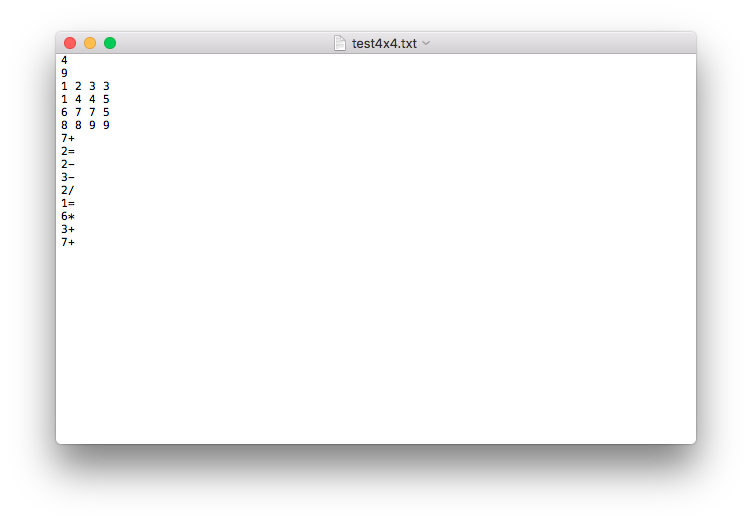
\includegraphics[scale=1]{Gambar/Perancangan/PerancanganInput.png}
\caption[Contoh \textit{file} masukan.]{Contoh \textit{file} masukan.}
\label{fig:perancanganmasukan}
\end{figure}

Adapun rincian dari \textit{file} teks masukan tersebut adalah sebagai berikut:

\begin{enumerate}
\item Baris pertama berisi ukuran \textit{grid} dan banyaknya \textit{cage} dari teka-teki Calcudoku tersebut. Angka pertama adalah ukuran \textit{grid}, dan angka kedua adalah banyaknya \textit{cage}.
\item Baris kedua sampai ke baris ke-\begin{math}2 + (n - 1)\end{math}, dengan \begin{math}n\end{math} adalah ukuran \textit{grid}, berisi matriks \textit{cage assignment}. Matriks ini merepresentasikan posisi dari setiap \textit{cage} dalam \textit{grid}. Setiap \textit{cage} direpresentasikan dengan angka yang berbeda. Setiap \textit{cage} dapat mempunyai ukuran (jumlah sel yang terdapat dalam \textit{cage}) yang bervariasi. Setiap sel dalam sebuah \textit{cage} harus berhubungan secara horizontal atau vertikal dengan sel lain dalam \textit{cage} yang sama.
\item Baris ke-\begin{math}2 + n\end{math} dan seterusnya berisi \textit{cage objectives} untuk setiap \textit{cage}. \textit{Cage objectives} berisikan angka tujuan dan operasi matematika yang telah ditentukan. Angka-angka dalam sebuah \textit{cage} harus mencapai angka tujuan jika dihitung menggunakan operasi matematika yang telah ditentukan.
\end{enumerate}

\section{Perancangan Keluaran}
\label{sec:perancangankeluaran}

Keluaran untuk perangkat lunak permainan teka-teki Calcudoku ini berupa sebuah matriks yang berisi solusi dari teka-teki Calcudoku yang sudah diselesaikan oleh program, seperti dapat dilihat pada Gambar~\ref{fig:perancangankeluaran}.

\begin{figure}
\centering
\captionsetup{justification=centering}
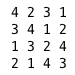
\includegraphics[scale=1]{Gambar/Perancangan/PerancanganOutput.png}
\caption[Contoh keluaran.]{Contoh keluaran.}
\label{fig:perancangankeluaran}
\end{figure}

\section{Perancangan Antarmuka}
\label{sec:perancanganantarmuka}

Antarmuka untuk perangkat lunak ini terdiri dari sebuah \textit{frame} yang berisi sebuah menu \textit{bar} dan GUI dari permainan teka-teki Calcudoku. GUI hanya akan ditampilkan jika perangkat lunak sudah membuka \textit{file} permainan. Jika \textit{file} permainan ditutup, maka GUI juga akan ditutup.

Gambar~\ref{fig:perancangangui1} menunjukkan perancangan GUI sebelum \textit{file} permainan dibuka. Gambar~\ref{fig:perancangangui2} menunjukkan perancangan GUI sesudah \textit{file} permainan dibuka. Gambar~\ref{fig:perancangangui3} menunjukkan perancangan GUI sesudah permainan berdasarkan \textit{file} permainan yang dibuka diselesaikan.

\begin{figure}
\centering
\captionsetup{justification=centering}
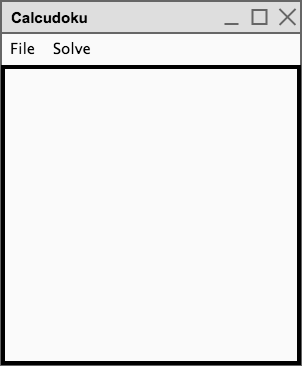
\includegraphics[scale=0.5]{Gambar/Perancangan/PerancanganGUI1.png}
\caption[Perancangan GUI sebelum \textit{file} permainan dibuka.]{Perancangan GUI sebelum membuka \textit{file} permainan}
\label{fig:perancangangui1}
\end{figure}

\begin{figure}
\centering
\captionsetup{justification=centering}
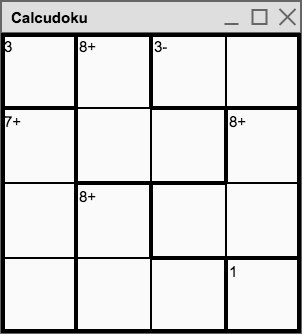
\includegraphics[scale=0.5]{Gambar/Perancangan/PerancanganGUI2.png}
\caption[Perancangan GUI sesudah \textit{file} permainan dibuka.]{Perancangan GUI sesudah membuka \textit{file} permainan}
\label{fig:perancangangui2}
\end{figure}

\begin{figure}
\centering
\captionsetup{justification=centering}
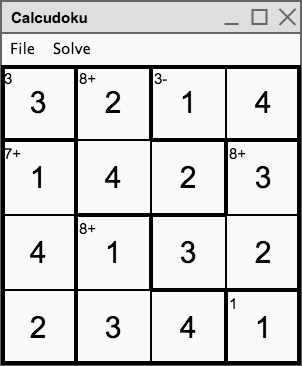
\includegraphics[scale=0.5]{Gambar/Perancangan/PerancanganGUI3.png}
\caption[Perancangan GUI sesudah permainan berdasarkan \textit{file} permainan yang dibuka diselesaikan.]{Perancangan GUI sesudah permainan berdasarkan \textit{file} permainan yang dibuka diselesaikan.}
\label{fig:perancangangui3}
\end{figure}

\clearpage

Menu \textit{bar} untuk perangkat lunak ini terdiri dari dua menu, yaitu:
\begin{enumerate}
\item \textit{File}, yaitu menu yang berisi \textit{item-item} menu yang terkait dengan \textit{file} permainan.
\item \textit{Solve}, yaitu menu yang berisi \textit{item-item} menu yang terkait dengan \textit{solver}.
\end{enumerate}

Menu \textit{File} mempunyai beberapa menu \textit{item}, yaitu:
\begin{enumerate}
\item \textit{Load Puzzle File}, yaitu menu \textit{item} untuk membuka \textit{file} permainan.
\item \textit{Reset Puzzle}, yaitu menu \textit{item} untuk me-\textit{reset} permainan.
\item \textit{Close Puzzle File}, yaitu menu \textit{item} untuk menutup \textit{file} permainan.
\item \textit{Check Puzzle}, yaitu menu \textit{item} untuk memeriksa permainan jika ada masukan yang salah di dalam \textit{grid}.
\item \textit{Exit}, yaitu menu \textit{item} untuk menutup perangkat lunak.
\end{enumerate}

Gambar~\ref{fig:perancanganguimenufile} menunjukkan isi dari menu \textit{File}.

\begin{figure}
\centering
\captionsetup{justification=centering}
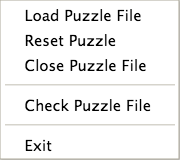
\includegraphics[scale=0.5]{Gambar/Perancangan/PerancanganGUIMenuFile.png}
\caption[Menu \textit{File}]{Menu \textit{File}}
\label{fig:perancanganguimenufile}
\end{figure}

Menu \textit{Solve} mempunyai beberapa menu \textit{item}, yaitu:
\begin{enumerate}
\item \textit{Backtracking}, yaitu menu \textit{item} untuk menyelesaikan permainan berdasarkan \textit{file} permainan yang dibuka dengan algoritma \textit{backtracking}.
\item \textit{Hybrid Genetic}, yaitu menu \textit{item} untuk menyelesaikan permainan berdasarkan \textit{file} permainan yang dibuka dengan algoritma \textit{hybrid genetic}.
\item \textit{Set Genetic Algorithm Parameters}, yaitu menu \textit{item} untuk mengatur nilai dari parameter-parameter untuk algoritma genetik.
\end{enumerate}

Gambar~\ref{fig:perancanganguimenusolve} menunjukkan isi dari menu \textit{Solve}.

\begin{figure}
\centering
\captionsetup{justification=centering}
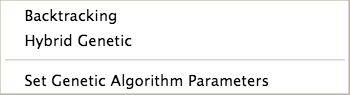
\includegraphics[scale=0.5]{Gambar/Perancangan/PerancanganGUIMenuSolve.png}
\caption[Menu \textit{Solve}]{Menu \textit{Solve}}
\label{fig:perancanganguimenusolve}
\end{figure}

\section{Diagram Kelas}
\label{sec:diagramkelas}

Perangkat lunak teka-teki Calcudoku ini terdiri dari beberapa kelas, yang dikelompokkan dalam tiga package, yaitu:

\begin{enumerate}
\item Model, yaitu \textit{engine} dari perangkat lunak ini. Package ini memiliki beberapa kelas, yaitu:
	\begin{enumerate}
	\item Grid, yaitu kelas yang merepresentasikan \textit{grid} dalam teka-teki Calcudoku.
	\item Cell, yaitu kelas yang merepresentasikan sel dalam teka-teki Calcudoku.
	\item Cage, yaitu kelas yang merepresentasikan \textit{cage} dalam teka-teki Calcudoku.
	\item SolverBacktracking, yaitu kelas \textit{solver} untuk teka-teki Calcudoku menggunakan algoritma backtracking.
	\item SolverHybridGenetic, yaitu kelas \textit{solver} untuk teka-teki Calcudoku menggunakan algoritma \textit{hybrid genetic}. Algoritma ini akan mencoba menyelesaikan teka-teki Calcudoku menggunakan algoritma \textit{rule based} terlebih dahulu. Algoritma genetik baru akan dijalankan jika algoritma \textit{rule based} gagal dalam menyelesaikan teka-teki Calcudoku.
	\item SolverRuleBased, yaitu kelas \textit{solver} untuk teka-teki Calcudoku menggunakan algoritma \textit{rule based}. Dalam algoritma \textit{hybrid genetic}, algoritma akan mencoba menyelesaikan teka-teki Calcudoku menggunakan algoritma \textit{rule based} terlebih dahulu.
	\item SolverGenetic, yaitu kelas \textit{solver} untuk teka-teki Calcudoku menggunakan algoritma genetik. Dalam algoritma \textit{hybrid genetic}, algoritma genetik baru akan dijalankan jika algoritma \textit{rule based} gagal dalam menyelesaikan teka-teki Calcudoku.
	\item Chromosome, yaitu kelas yang merepresentasikan sebuah kromosom untuk algoritma genetik dalam solver \textit{hybrid genetic}.
	\item ChromosomeComparator, yaitu kelas pembanding \textit{custom} (\textit{custom comparator}) yang berfungsi untuk mengurutkan kromosom berdasarkan nilai kelayakkannya (\textit{fitness value}).	
	\end{enumerate}
\item View, yaitu GUI dari perangkat lunak ini. Package ini memiliki beberapa kelas, yaitu:
	\begin{enumerate}
	\item Calcudoku, yaitu kelas \textit{frame} yang berisi menu \textit{bar} dan instansiasi kelas panel GUI.
	\item WindowListener, yaitu kelas \textit{listener} untuk kelas Calcudoku. \textit{Listener} ini berfungsi untuk menambahkan pesan peringatan saat akan menutup perangkat lunak.
	\item PuzzleFileFilter, yaitu kelas filter untuk \textit{file chooser}. Filter ini membatasi agar \textit{file chooser} hanya bisa membuka \textit{file} teks.
	\item GUI, yaitu kelas panel yang merepresentasikan GUI dari permainan teka-teki Calcudoku.
	\item CellKeyListener, yaitu kelas \textit{listener} untuk kelas GUI. \textit{Listener} ini berfungsi untuk menggerakkan kursor dari sebuah sel ke sel di sebelahnya menggunakan tombol-tombol panah ke kiri, ke atas, ke bawah, dan ke kanan. Listener ini juga berfungsi untuk membatasi agar sel hanya bisa diisi oleh satu angka.
	\item PopupMenuListener, yaitu kelas \textit{listener} untuk kelas GUI. \textit{Listener} ini berfungsi untuk mengisi sel dengan angka menggunakan menu \textit{pop up}, sel akan diisi dengan angka yang dipilih.
	\item CellTextFieldListener, yaitu kelas \textit{listener} untuk kelas GUI. \textit{Listener} ini berfungsi untuk mengisikan sel dalam kelas Grid dengan angka yang diisikan ke dalam sel dalam GUI.
	\item GeneticParameterss, yaitu kelas yang berisi \textit{form} untuk mengatur nilai dari parameter-parameter untuk algoritma genetik.
	\end{enumerate}
\item Controller, yaitu penghubung antara \textit{package} model dan \textit{package} view. Package ini hanya berisi satu kelas, yaitu kelas Controller.
\end{enumerate}

Diagram kelas untuk perangkat lunak ini dapat dilihat pada Gambar~\ref{fig:diagramkelas}.

\begin{figure}
\centering
\captionsetup{justification=centering}
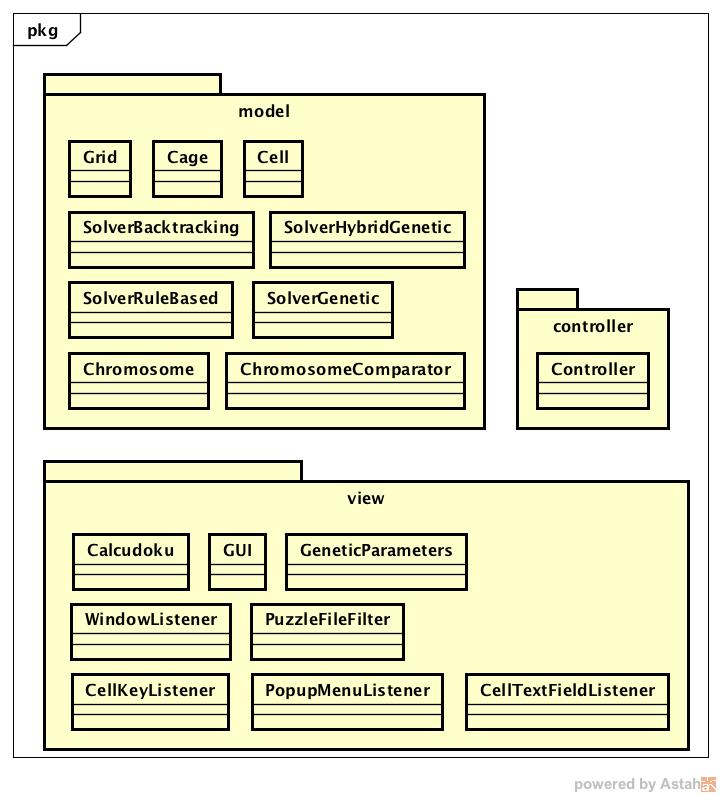
\includegraphics[scale=0.5]{Gambar/Perancangan/DiagramKelas.jpg}
\caption[Diagram kelas untuk perangkat lunak Calcudoku.]{Diagram kelas untuk perangkat lunak Calcudoku.}
\label{fig:diagramkelas}
\end{figure}

Berikut ini adalah rincian dari setiap kelas, dengan setiap atribut dan setiap \textit{method} yang dimilikinya.

\subsection{Kelas Grid}
\label{sec:kelasgrid}

Kelas Grid mempunyai beberapa atribut, yaitu:

\begin{enumerate}
\item size, yaitu ukuran dari matriks \textit{grid}.
\item numberOfCages, yaitu banyaknya \textit{cage} yang terdapat dalam \textit{grid}.
\item cageCells, yaitu sebuah matriks \textit{cage assignment}. Matriks ini merepresentasikan posisi dari setiap \textit{cage} dalam \textit{grid}.
\item cageObjectives, yaitu sebuah \textit{array} yang berisi \textit{cage objectives} untuk setiap \textit{cage}. \textit{Cage objectives} berisikan angka tujuan dan operasi matematika yang telah ditentukan.
\item grid, yaitu representasi dari \textit{grid} dalam teka-teki Calcudoku. grid adalah sebuah matriks yang berisi sel-sel. Matriks ini berukuran \begin{math} n \times n\end{math}.
\item cages, yaitu representasi dari sebuah \textit{cage} dalam sebuah \textit{grid}.
\end{enumerate}

Kelas Grid mempunyai beberapa \textit{method}, yaitu:

\begin{enumerate}
\item Grid(Integer size, Integer numberOfCages, Integer[][] cageCells, String[] cageObjectives), yaitu konstruktor dari kelas ini. Konstruktor ini menerima masukan berupa ukuran dari matriks \textit{grid}, banyaknya \textit{cage} yang terdapat dalam \textit{grid}, matriks \textit{cage assignment}, dan array \textit{cage objectives}.
\item countAreas(Integer[][] array), yaitu \textit{method} pembungkus dari \textit{method} countAreas(int[][] array, boolean[][] checked). \textit{Method} ini menerima masukan berupa array \textit{cage assignment} untuk sebuah \textit{cage}, dan menghasilkan keluaran berupa jumlah area dari \textit{cage} tersebut.
\item countAreas(Integer[][] array, boolean[][] checked), yaitu \textit{method} yang menghitung jumlah area dari sebuah \textit{cage} secara rekursif dengan menggunakan algoritma \textit{flood fill}. \textit{Method} ini menerima masukan berupa array \textit{cage assignment} untuk sebuah \textit{cage} dan sebuah array checked yang berfungsi untuk menandai sel-sel yang sudah pernah dikunjungi atau belum, dan menghasilkan keluaran berupa jumlah area dari \textit{cage} tersebut.
\item floodFill(int i, int j, Integer[][] array, boolean[][] checked), yaitu implementasi dari algoritma \textit{flood fill} untuk menghitung jumlah area dari sebuah \textit{cage}. \textit{Method} ini menerima masukan berupa posisi baris dan kolom dari sebuah sel, array \textit{cage assignment} untuk sebuah \textit{cage} dan sebuah array checked yang berfungsi untuk menandai sel-sel yang sudah pernah dikunjungi atau belum.
\item isCageCellsSizeValid(Integer[][] cageCells), yaitu \textit{method} yang memeriksa apakah ukuran matriks \textit{cage assignment} valid atau tidak. \textit{Method} ini menerima masukan berupa matriks \textit{cage assignment}, dan menghasilkan keluaran apakah matriks tersebut \textit{valid} atau tidak. Matriks tersebut \textit{valid} jika ukuran barisnya dan kolomnya sama dengan variabel size.
\item isCageObjectivesSizeValid(String[] cageObjectives), yaitu \textit{method} yang memeriksa apakah ukuran matriks \textit{cage objectives} valid atau tidak. \textit{Method} ini menerima masukan berupa \textit{array cage objectives}, dan menghasilkan keluaran apakah \textit{array} tersebut \textit{valid} atau tidak. Array tersebut \textit{valid} jika ukuran dari \textit{array} tersebut sama dengan variabel numberOfCages.
\item isCageAssignmentValid(Integer[][] array), yaitu \textit{method} yang memeriksa apakah \textit{cage assignment} untuk sebuah \textit{cage valid} atau tidak. \textit{Method} ini menerima masukan berupa matriks \textit{cage assignment} untuk sebuah \textit{cage} dan menghasilkan keluaran apakah matriks tersebut atau tidak. Matriks tersebut \textit{valid} jika jumlah area dari \textit{cage} tersebut adalah satu.
\item isCagesValid(Cage[] cages), yaitu \textit{method} yang memeriksa apakah setiap \textit{cage} yang ada di dalam \textit{grid valid} atau tidak. \textit{Method} ini menerima masukan berupa \textit{array cage}, dan menghasilkan keluaran apakah \textit{array} tersebut \textit{valid} atau tidak. \textit{Array} tersebut \textit{valid} jika setiap \textit{cage} dengan operator = hanya berukuran satu sel, setiap \textit{cage} dengan operator + atau \begin{math}\times\end{math} berukuran minimal dua sel, dan setiap \textit{cage} dengan operator - atau \begin{math}\div\end{math} berukuran tepat dua sel.
\item generateCages(Cage[] cages), yaitu \textit{method} yang membangkitkan \textit{cage-cage} dalam sebuah \textit{grid}. \textit{Method} ini menerima masukan berupa sebuah array \textit{Cage} yang kosong.
\item generateGrid(Cell[][] grid, Cage[] cages), yaitu \textit{method} yang membangkitkan \textit{grid} dan \textit{cage assignment} dari \textit{grid} tersebut.. \textit{Method} ini menerima masukan berupa sebuah matriks sel yang kosong dan sebuah array \textit{cage} yang kosong.
\item getRow(int rowNumber), yaitu \textit{method} untuk mendapatkan isi dari sebuah baris yang diminta. \textit{Method} ini menerima masukan berupa nomor baris yang diminta dan menghasilkan keluaran berupa isi baris yang diminta.
\item getColumn(int columnNumber), yaitu \textit{method} untuk mendapatkan isi dari sebuah kolom yang diminta. \textit{Method} ini menerima masukan berupa nomor kolom yang diminta dan menghasilkan keluaran berupa isi kolom yang diminta dalam bentuk ArrayList.
\item getCageValues(int cageNumber), yaitu \textit{method} untuk mendapatkan isi dari sebuah \textit{cage} yang diminta. \textit{Method} ini menerima masukan berupa nomor \textit{cage} yang diminta dan menghasilkan keluaran berupa isi \textit{cage} yang diminta dalam bentuk ArrayList.
\item isArrayValid(ArrayList<Integer> array), yaitu \textit{method} untuk memeriksa apakah sebuah \textit{array valid} atau tidak. \textit{Method} ini menerima masukan berupa \textit{array} yang akan diperiksa dan menghasilkan keluaran apakah \textit{array} tersebut \textit{valid} atau tidak. \textit{Array} tersebut \textit{valid} jika tidak ada angka yang berulang dalam \textit{array} tersebut.
\item isRowValid(int row), yaitu \textit{method} untuk memeriksa apakah sebuah baris \textit{valid} atau tidak. \textit{Method} ini menerima masukan berupa nomor baris yang diminta dan menghasilkan keluaran apakah baris yang diminta tersebut \textit{valid} atau tidak. Baris tersebut \textit{valid} jika tidak ada angka yang berulang dalam baris tersebut.
\item solverIsRowValid(int column), yaitu \textit{method} yang sama dengan isRowValid, tetapi \textit{method} ini hanya untuk dipanggil oleh solver.
\item isColumnValid(int column), yaitu \textit{method} untuk memeriksa apakah sebuah kolom \textit{valid} atau tidak. \textit{Method} ini menerima masukan berupa nomor kolom yang diminta dan menghasilkan keluaran apakah kolom yang diminta tersebut \textit{valid} atau tidak. Kolom tersebut \textit{valid} jika tidak ada angka yang berulang dalam kolom tersebut.
\item solverIsColumnValid(int column), yaitu \textit{method} yang sama dengan isColumnValid, tetapi \textit{method} ini hanya untuk dipanggil oleh solver.
\item isCageValuesValid(int cageNumber), yaitu \textit{method} untuk memeriksa apakah nilai dari setiap sel yang berada dalam sebuah \textit{cage valid} atau tidak. \textit{Method} ini menerima masukan berupa nomor \textit{cage} yang diminta dan menghasilkan keluaran apakah nilai dari setiap sel yang berada dalam \textit{cage} yang diminta tersebut \textit{valid} atau tidak. \textit{Cage} tersebut \textit{valid} jika nilai dari setiap sel yang berada di dalam \textit{cage} tersebut mencapai angka tujuan yang telah ditentukan jika dihitung menggunakan operator yang telah ditentukan.
\item isCageValid(int row, int column), yaitu \textit{method} untuk memeriksa apakah sebuah \textit{cage valid} atau tidak. \textit{Method} ini menerima masukan berupa nomor baris dan nomor kolom dari sebuah sel yang diminta dan menghasilkan keluaran apakah \textit{cage} yang berisi sel tersebut \textit{valid} atau tidak. \textit{Cage} tersebut \textit{valid} jika angka-angka dalam \textit{cage} tersebut mencapai angka tujuan yang telah ditentukan jika dihitung menggunakan operator yang telah ditentukan.
\item solverIsCageValid(int column), yaitu \textit{method} yang sama dengan isCageValid, tetapi \textit{method} ini hanya untuk dipanggil oleh solver.
\item isCellValueValid(int row, int column), yaitu \textit{method} untuk memeriksa apakah nilai dari sel tersebut \textit{valid} atau tidak. \textit{Method} ini menerima masukan berupa nomor baris dan nomor kolom dari sel yang akan diperiksa dan menghasilkan keluaran apakah nilai dari sel tersebut \textit{valid} atau tidak. Nilai dari sebuah sel \textit{valid} jika nilai dari sel tersebut tidak berulang dalam baris dan kolom tempat sel tersebut berada, dan angka-angka dari \textit{cage} yang berisi sel tersebut mencapai angka tujuan yang telah ditentukan jika dihitung menggunakan operator yang telah ditentukan.
\item solverIsCellValueValid(int column), yaitu \textit{method} yang sama dengan isCellValueValid, tetapi \textit{method} ini hanya untuk dipanggil oleh solver.
\item setCellValue(int row, int column, Integer value), yaitu \textit{method} untuk mengisi sebuah sel dengan nilai yang telah ditentukan. \textit{Method} ini menerima masukan berupa nomor baris dan nomor kolom dari sel yang akan diisi dan nilai dari sel tersebut, dan menghasilkan keluaran apakah nilai dari sel tersebut \textit{valid} atau tidak. Nilai dari sebuah sel \textit{valid} jika nilai dari sel tersebut tidak berulang dalam baris dan kolom tempat sel tersebut berada, dan angka-angka dari \textit{cage} yang berisi sel tersebut mencapai angka tujuan yang telah ditentukan jika dihitung menggunakan operator yang telah ditentukan.
\item solverSetCellValue(int row, int column, Integer value), yaitu \textit{method} yang sama dengan setCellValue, tetapi \textit{method} ini hanya untuk dipanggil oleh solver.
\item unsetCellValue(int row, int column), yaitu \textit{method} untuk menghapus isi dari sebuah sel. \textit{Method} ini menerima masukan berupa nomor baris dan nomor kolom dari sel yang akan dihapus isinya.
\item isWin(), yaitu \textit{method} yang memeriksa apakah semua sel sudah diisi dengan nilai yang \textit{valid} atau tidak. \textit{Method} ini menghasilkan keluaran apakah semua sel sudah diisi dengan nilai yang \textit{valid} atau tidak. \textit{Method} ini menghasilkan \textit{null} jika ada sel yang belum diisi.
\item checkGrid(), yaitu \textit{method} yang memeriksa apakah ada sel yang berisi nilai yang tidak \textit{valid} atau tidak. \textit{Method} ini akan menghasilkan apakah ada sel yang berisi nilai yang tidak \textit{valid} atau tidak. Nilai dari sebuah sel \textit{valid} jika nilai dari sel tersebut tidak berulang dalam baris dan kolom tempat sel tersebut berada, dan angka-angka dari \textit{cage} yang berisi sel tersebut mencapai angka tujuan yang telah ditentukan jika dihitung menggunakan operator yang telah ditentukan. \textit{Method} ini juga memeriksa apakah ada sel yang kosong atau tidak.
\item isFilled(), yaitu \textit{method} yang memeriksa apakah semua sel sudah diisi atau tidak. \textit{Method} ini menghasilkan keluaran apakah semua sel sudah diisi atau tidak.
\item getCellValue(int row, int column), yaitu \textit{method} untuk mendapatkan isi dari sebuah sel. \textit{Method} ini menerima masukan berupa nomor baris dan nomor kolom dari sel yang diminta dan menghasilkan keluaran berupa isi dari sel yang diminta tersebut.
\item getSize(), yaitu \textit{method} untuk mendapatkan ukuran dari \textit{grid}. \textit{Method} ini menghasilkan keluaran berupa ukuran dari \textit{grid}.
\item getNumberOfCages(), yaitu \textit{method} untuk mendapatkan jumlah \textit{cage} yang ada di dalam \textit{grid}. \textit{Method} ini menghasilkan keluaran berupa jumlah \textit{cage} yang ada di dalam \textit{grid}.
\item getCageCells(), yaitu \textit{method} untuk mendapatkan matriks \textit{cage assignment} dari \textit{grid}. \textit{Method} ini menghasilkan keluaran berupa matriks \textit{cage assignment} dari \textit{grid}.
\item getCageObjectives(), yaitu \textit{method} untuk mendapatkan \textit{cage objectives} dari setiap \textit{cage} dalam \textit{grid}. \textit{Method} ini menghasilkan keluaran berupa sebuah array yang berisi \textit{cage objectives} dari setiap \textit{cage} dalam \textit{grid}.
\item getGridContents(), yaitu \textit{method} untuk mendapatkan nilai dari setiap sel \textit{grid}. \textit{Method} ini menghasilkan keluaran berupa sebuah matriks yang berisi nilai dari setiap sel \textit{grid}.
\item getCages(), yaitu \textit{method} untuk mendapatkan semua \textit{cage} dalam \textit{grid}. \textit{Method} ini menghasilkan keluaran berupa array yang berisi semua \textit{cage} dalam \textit{grid}.
\item getGame(), yaitu \textit{method} untuk mendapatkan instansiasi saat ini dari kelas \textit{Grid}. \textit{Method} ini menghasilkan keluara berupa instansiasi saat ini dari kelas \textit{Grid}.
\end{enumerate}

Diagram kelas Grid dapat dilihat pada Gambar~\ref{fig:diagramkelasgrid}.

\begin{figure}
\centering
\captionsetup{justification=centering}
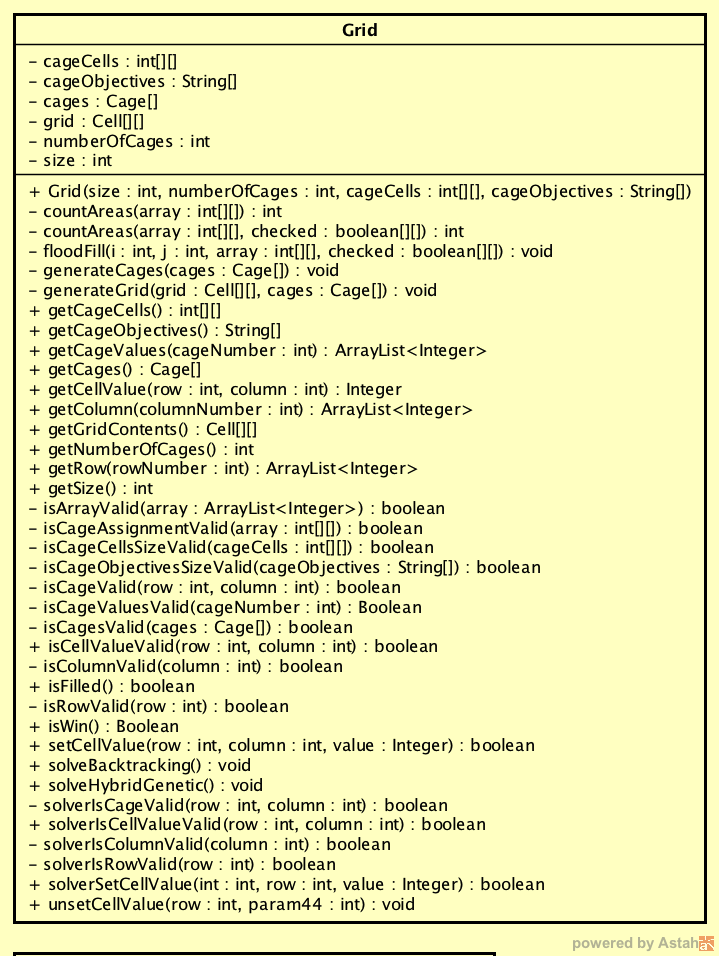
\includegraphics[scale=0.5]{Gambar/Perancangan/DiagramKelasGrid.png}
\caption[Diagram kelas Grid.]{Diagram kelas Grid.}
\label{fig:diagramkelasgrid}
\end{figure}

\subsection{Kelas Cage}
\label{sec:kelascage}

Kelas Cage mempunyai beberapa atribut, yaitu:

\begin{enumerate}
\item objective, yaitu angka tujuan dan operator yang ditentukan untuk \textit{cage} tersebut.
\item targetNumber, yaitu angka tujuan dari \textit{cage} tersebut.
\item operator, yaitu operator yang ditentukan untuk \textit{cage} tersebut.
\item cells, yaitu sebuah array yang berisi sel-sel yang merupakan anggota dari \textit{cage} tersebut.
\end{enumerate}

Kelas Cage mempunyai \textit{method-method} berikut:

\begin{enumerate}
\item Cage(String objectives), yaitu konstruktor dari kelas ini. Konstruktor ini menerima masukan berupa \textit{cage objectives} dari \textit{cage} tersebut.
\item isCageObjectiveValid(String cageObjective), yaitu \textit{method} yang memeriksa apakah \textit{cage objective} dari \textit{cage} tersebut \textit{valid} atau tidak. \textit{Method} ini menerima masukan berupa String yang berisi \textit{cage objective} dan menghasilkan keluaran apakah String tersebut valid atau tidak. \textit{Cage objective valid} jika isi dari \textit{cage objective} tersebut adalah satu angka tujuan dari \textit{cage} tersebut dan diikuti oleh satu operator yang telah ditentukan untuk \textit{cage} tersebut.
\item generateTargetNumber(String objective), yaitu \textit{method} yang membangkitkan angka tujuan dari sebuah \textit{cage} dari \textit{cage objective} yang diberikan. \textit{Method} ini menerima masukan berupa String yang berisi \textit{cage objective} dari sebuah \textit{cage} dan menghasilkan keluaran berupa angka tujuan dari \textit{cage} tersebut.
\item generateOperator(String objective), yaitu \textit{method} yang membangkitkan operator yang telah ditentukan untuk sebuah \textit{cage} dari \textit{cage objective} yang diberikan. \textit{Method} ini menerima masukan berupa String yang berisi \textit{cage objective} dari sebuah \textit{cage} dan menghasilkan keluaran berupa operator yang telah ditentukan untuk \textit{cage} tersebut.
\item addCell(Cell c), yaitu \textit{method} untuk menambahkan sebuah sel kedalam sebuah \textit{cage}. \textit{Method} ini menerima masukan berupa sel yang akan dimasukkan ke dalam \textit{cage}.
\item isCageContainsNull(), yaitu \textit{method} yang memeriksa apakah sebuah \textit{cage} mempunyai sel yang belum diisi. \textit{Method} ini menghasilkan keluaran apakah \textit{cage} tersebut mempunyai sel yang belum terisi.
\item isCageValuesValid(), yaitu \textit{method} yang memeriksa apakah angka-angka dalam sebuah \textit{cage} mencapai angka tujuan dari \textit{cage} tersebut jika dihitung menggunakan operator yang telah ditentukan untuk \textit{cage} tersebut. \textit{Method} ini menghasilkan keluaran apakah angka-angka dalam \textit{cage} tersebut mencapai angka tujuan dari \textit{cage} tersebut jika dihitung menggunakan operator yang telah ditentukan untuk \textit{cage} tersebut. \textit{Method} ini menghasilkan \textit{null} jika ada sel di dalam \textit{cage} yang belum diisi.
\item countValue(), yaitu \textit{method} yang menghitung angka-angka di dalam sebuah \textit{cage} menggunakan operator yang telah ditentukan untuk \textit{cage} tersebut. \textit{Method} ini menghasilkan keluaran hasil perhitungan dari angka-angka di dalam sebuah \textit{cage} menggunakan operator yang telah ditentukan untuk \textit{cage} tersebut. \textit{Method} ini menghasilkan \textit{null} jika ada sel di dalam \textit{cage} yang belum diisi.
\item getTargetNumber(), yaitu \textit{method} untuk mendapatkan angka tujuan dari sebuah \textit{cage}. \textit{Method} ini menghasilkan keluaran berupa angka tujuan dari \textit{cage} tersebut.
\item getOperator(), yaitu \textit{method} untuk mendapatkan operator yang telah ditentukan untuk sebuah \textit{cage}. \textit{Method} ini menghasilkan keluaran berupa operator yang telah ditentukan untuk \textit{cage} tersebut.
\item getCells(), yaitu \textit{method} untuk mendapatkan sel-sel anggota sebuah \textit{cage}. \textit{Method} ini menghasilkan keluaran sebuah ArrayList yang berisi sel-sel anggota \textit{cage} tersebut.
\item getSize(), yaitu \textit{method} untuk mendapatkan jumlah dari sel-sel anggota sebuah \textit{cage}. \textit{Method} ini menghasilkan keluaran berupa jumlah dari sel-sel anggota \textit{cage} tersebut.
\end{enumerate}

Diagram kelas Cage dapat dilihat pada Gambar~\ref{fig:diagramkelascage}.

\begin{figure}
\centering
\captionsetup{justification=centering}
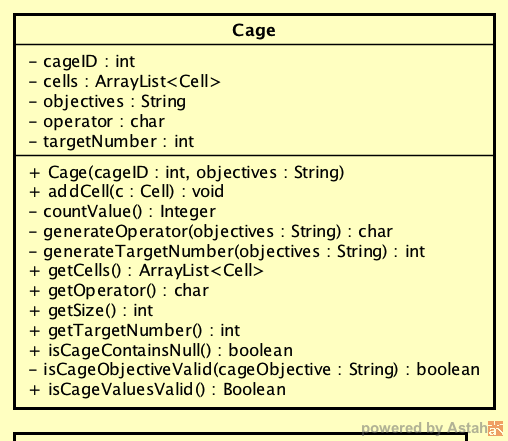
\includegraphics[scale=0.5]{Gambar/Perancangan/DiagramKelasCage.png}
\caption[Diagram kelas Cage.]{Diagram kelas Cage.}
\label{fig:diagramkelascage}
\end{figure}

\subsection{Kelas Cell}
\label{sec:kelascell}

Kelas Cell mempunyai beberapa atribut, yaitu:

\begin{enumerate}
\item row, yaitu posisi baris dari sel tersebut.
\item column, yaitu posisi kolom dari sel tersebut.
\item cageID, yaitu nomor \textit{cage} yang berisi sel tersebut.
\item value, yaitu nilai dari sel tersebut.
\end{enumerate}

Kelas Cell mempunyai beberapa \textit{method}, yaitu:

\begin{enumerate}
\item Cell(int row, int column, int cageID), yaitu konstruktor dari kelas ini. Konstruktor ini menerima masukan berupa nomor baris, dan nomor kolom dari sel tersebut, dan nomor \textit{cage} yang berisi sel tersebut.
\item setValue(Integer value), yaitu \textit{method} untuk mengisi sebuah sel tersebut dengan nilai yang telah ditentukan. \textit{Method} ini menerima masukan berupa nilai yang akan diisikan ke dalam sel tersebut.
\item getValue(), yaitu \textit{method} untuk mendapatkan nilai dari sel tersebut. \textit{Method} ini menghasilkan keluaran berupa nilai dari sel tersebut.
\item getRow(), yaitu \textit{method} untuk mendapatkan nomor baris dari sebuah sel. \textit{Method} ini menghasilkan keluaran berupa nomor baris dari sel tersebut.
\item getColumn(), yaitu \textit{method} untuk mendapatkan nomor kolom dari sebuah sel. \textit{Method} ini menghasilkan keluaran berupa nomor kolom dari sel tersebut.
\item getCageID(), yaitu \textit{method} untuk mendapatkan nomor \textit{cage} yang berisi sebuah sel. \textit{Method} ini menghasilkan keluaran berupa nomor \textit{cage} yang berisi sel tersebut.
\end{enumerate}

Diagram kelas Cell dapat dilihat pada Gambar~\ref{fig:diagramkelascell}.

\begin{figure}
\centering
\captionsetup{justification=centering}
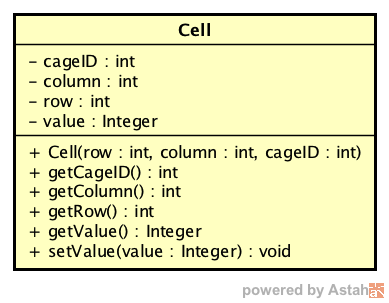
\includegraphics[scale=0.5]{Gambar/Perancangan/DiagramKelasCell.png}
\caption[Diagram kelas Cell.]{Diagram kelas Cell.}
\label{fig:diagramkelascell}
\end{figure}

\subsection{Kelas SolverBacktracking}
\label{sec:kelassolverbt}

Kelas SolverBacktracking mempunyai beberapa atribut, yaitu:

\begin{enumerate}
\item grid, yaitu \textit{grid} yang akan diselesaikan oleh \textit{solver} dengan algoritma \textit{backtracking}.
\item size, yaitu ukuran dari \textit{grid} yang akan diselesaikan oleh \textit{solver} dengan algoritma \textit{backtracking}.
\item solution, yaitu \textit{grid} yang sudah diselesaikan oleh \textit{solver} dengan algoritma \textit{backtracking}.
\end{enumerate}

Kelas SolverBacktracking mempunyai beberapa \textit{method}, yaitu:

\begin{enumerate}
\item SolverBacktracking(Grid grid), yaitu konstruktor dari kelas ini. Konstruktor ini menerima masukan berupa \textit{grid} yang akan diselesaikan oleh \textit{solver} dengan algoritma \textit{backtracking}.
\item solve(), yaitu \textit{method} pembungkus dari \textit{method} solve(int row, int column). \textit{Method} ini menghasilkan keluaran apakah \textit{solver} berhasil menyelesaikan teka-teki Calcudoku atau tidak. \textit{Solver} bekerja mulai dari sel pada sudut kiri atas, lalu bergerak ke kanan sampai ke sel yang paling kanan, lalu bergerak ke baris berikutnya sampai ke baris yang paling bawah, selesai pada sel pada sudut kanan bawah.
\item solve(int row, int column), yaitu \textit{method} yang mencoba untuk menyelesaikan teka-teki Calcudoku menggunakan algoritma \textit{backtracking}. \textit{Method} ini menerima masukan berupa nomor baris dan nomor kolom yang akan diisi oleh \textit{solver} dan menghasilkan keluaran apakah nilai yang diisi oleh \textit{solver valid} atau tidak. \textit{Solver} akan mulai mengisi sel dari angka 1. Jika berhasil, maka \textit{solver} akan maju ke sel berikutnya. Jika gagal, maka \textit{solver} akan mencoba kemungkinan angka berikutnya. Jika semua kemungkinan angka gagal, maka \textit{solver} akan mundur ke sel sebelumnya dan mencoba kemungkinan angka berikutnya.
\item getGrid(), yaitu \textit{method} untuk mendapatkan \textit{grid}. \textit{Method} ini menghasilkan keluaran berupa \textit{grid}.
\item getSolution(), yaitu \textit{method} untuk mendapatkan solusi dari \textit{grid} yang sudah diselesaikan oleh \textit{solver}. \textit{Method} ini menghasilkan keluaran berupa solusi dari \textit{grid} tersebut.
\item printGrid(), yaitu \textit{method} untuk mencetak isi \textit{grid} ke layar. \textit{Method} ini menerima masukan berupa \textit{grid} yang akan dicetak isinya ke layar.
\end{enumerate}

Diagram kelas SolverBacktracking dapat dilihat pada Gambar~\ref{fig:diagramkelassolverbt}.

\begin{figure}
\centering
\captionsetup{justification=centering}
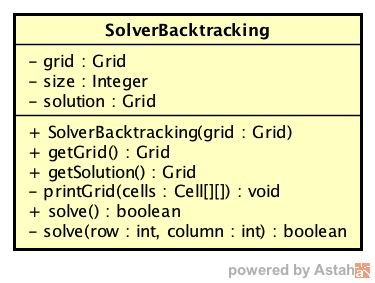
\includegraphics[scale=0.5]{Gambar/Perancangan/DiagramKelasSolverBacktracking.png}
\caption[Diagram kelas SolverBacktracking.]{Diagram kelas SolverBacktracking.}
\label{fig:diagramkelassolverbt}
\end{figure}

\subsection{Kelas SolverHybridGenetic}
\label{sec:kelassolverhg}

Kelas SolverHybridGenetic mempunyai beberapa atribut, yaitu:

\begin{enumerate}
\item grid, yaitu \textit{grid} yang akan diselesaikan oleh \textit{solver} dengan algoritma \textit{hybrid genetic}.
\item gridRuleBased, yaitu \textit{grid} yang telah diselesaikan oleh algoritma \textit{rule based}.
\item size, yaitu ukuran dari \textit{grid} yang akan diselesaikan oleh \textit{solver} dengan algoritma \textit{hybrid genetic}.
\item solution, yaitu \textit{grid} yang sudah diselesaikan oleh \textit{solver} dengan algoritma \textit{hybrid genetic}.
\item generations, yaitu jumlah generasi maksimum yang akan dibangkitkan oleh algoritma genetik.
\item populationSize, yaitu jumlah kromosom yang akan dibangkitkan dalam sebuah generasi.
\item elitismRate, yaitu parameter tingkat \textit{elitism} dalam algoritma genetik..
\item crossoverRate, yaitu parameter tingkat kawin silang dalam algoritma genetik.
\item mutationRate, yaitu parameter tingkat mutasi dalam algoritma genetik.
\end{enumerate}

Kelas SolverHybridGenetic mempunyai beberapa \textit{method}, yaitu:

\begin{enumerate}
\item SolverHybridGenetic(Grid grid, Integer generations, Integer populationSize, Double elitismRate, Double crossoverRate, Double mutationRate), yaitu konstruktor dari kelas ini. Konstruktor ini menerima masukan berupa \textit{grid} yang akan diselesaikan oleh \textit{solver} dengan algoritma \textit{hybrid genetic}, dan parameter-parameter algoritma genetik, yaitu jumlah generasi, jumlah populasi dalam sebuah generasi, tingkat \textit{elitism}, tingkat kawin silang, dan tingkat mutasi.
\item getGrid(), yaitu \textit{method} untuk mendapatkan \textit{grid} yang akan diselesaikan oleh \textit{solver} dengan algoritma \textit{hybrid genetic}.
\item getSolution(), yaitu \textit{method} untuk mendapatkan \textit{grid} yang sudah diselesaikan oleh \textit{solver} dengan algoritma \textit{hybrid genetic}.
\item solve(), yaitu \textit{method} yang mencoba untuk menyelesaikan teka-teki Calcudoku menggunakan algoritma \textit{hybrid genetic}. \textit{Method} ini akan memanggil solver algoritma \textit{rule based}. Jika algoritma \textit{rule based} gagal dalam menyelesaikan teka-teki Calcudoku, maka \textit{method} akan memanggil solver algoritma genetik. \textit{Method} ini menghasilkan keluaran apakah \textit{solver} berhasil menyelesaikan teka-teki Calcudoku atau tidak.
\item printGrid(), yaitu \textit{method} untuk mencetak isi \textit{grid} ke layar. \textit{Method} ini menerima masukan berupa \textit{grid} yang akan dicetak isinya ke layar.

\end{enumerate}

Diagram kelas SolverHybridGenetic dapat dilihat pada Gambar~\ref{fig:diagramkelassolverhg}.

\begin{figure}
\centering
\captionsetup{justification=centering}
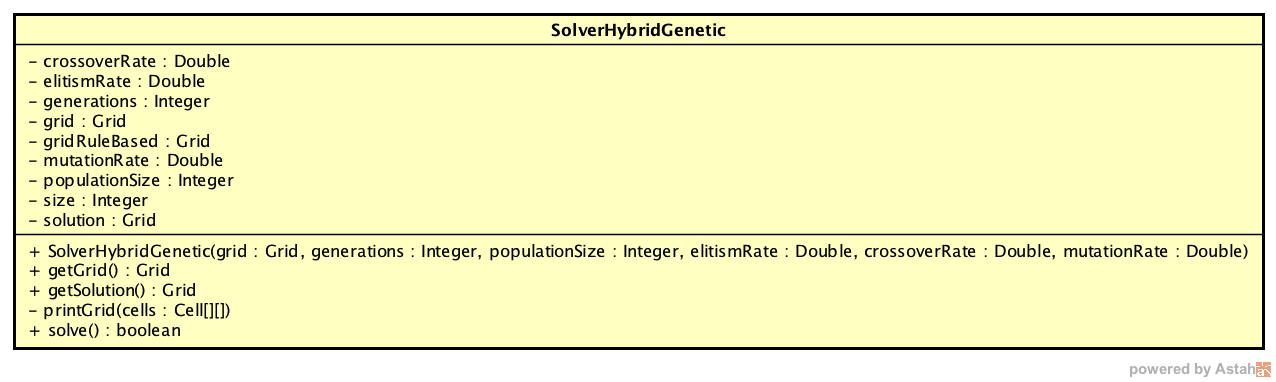
\includegraphics[scale=0.3]{Gambar/Perancangan/DiagramKelasSolverHybridGenetic.png}
\caption[Diagram kelas SolverHybridGenetic.]{Diagram kelas SolverHybridGenetic.}
\label{fig:diagramkelassolverhg}
\end{figure}

\subsection{Kelas SolverRuleBased}
\label{sec:kelassolverrb}

Kelas SolverRuleBased mempunyai beberapa atribut, yaitu:

\begin{enumerate}
\item grid, yaitu \textit{grid} yang akan diselesaikan oleh \textit{solver} dengan algoritma \textit{rule based}.
\item size, yaitu ukuran dari \textit{grid} yang akan diselesaikan oleh \textit{solver} dengan algoritma \textit{rule based}.
\item solution, yaitu \textit{grid} yang sudah diselesaikan oleh \textit{solver} dengan algoritma \textit{rule based}.
\item possibleValues, yaitu sebuah \textit{array} yang menampung semua kemungkinan angka yang mungkin untuk setiap sel yang ada di dalam \textit{grid}
\end{enumerate}

Kelas SolverRuleBased mempunyai \textit{method-method} berikut:

\begin{enumerate}
\item SolverRuleBased(Grid grid), yaitu konstruktor dari kelas ini. Konstruktor ini menerima masukan berupa \textit{grid} yang akan diselesaikan oleh \textit{solver} dengan algoritma \textit{rule based}, dan parameter-parameter algoritma genetik, yaitu jumlah generasi, jumlah populasi dalam sebuah generasi, tingkat \textit{elitism}, tingkat kawin silang, dan tingkat mutasi.
\item generatePossibleValuesArray(), yaitu \textit{method} yang membangkitkan kemungkinan angka-angka yang mungkin untuk setiap sel yang ada di dalam \textit{grid}. Angka-angka yang mungkin adalah dari 1 sampai ke ukuran dari \textit{grid}. \textit{Method} ini menghasilkan keluaran berupa array yang menampung semua kemungkinan angka yang mungkin untuk setiap sel yang ada di dalam \textit{grid}.
\item solve(), yaitu \textit{method} yang mencoba untuk menyelesaikan teka-teki Calcudoku menggunakan algoritma \textit{rule based}. \textit{Method} ini menghasilkan keluaran apakah \textit{solver} berhasil menyelesaikan teka-teki Calcudoku atau tidak. \textit{Solver} akan mencoba menyelesaikan teka-teki Calcudoku menggunakan aturan-aturan logika, misalnya \textit{single square rule}, \textit{killer combination rule}, \textit{naked subset rule}, \textit{hidden subset rule}, dan \textit{evil twin rule}. Aturan \textit{single square} dan \textit{killer combination} hanya dipakai sekali, dan dilakukan oleh \textit{method} ini, sedangkan aturan \textit{naked subset}, \textit{hidden subset}, dan \textit{evil twin} dapat dipakai berkali-kali, dan dilakukan oleh \textit{method} solveLoop().
\item solveLoop(), yaitu \textit{method} yang mengaplikasikan aturan \textit{naked subset}, \textit{hidden subset}, dan \textit{evil twin} kepada \textit{grid} yang sedang diselesaikan oleh algoritma \textit{rule based}. \textit{Method} ini menerima masukan berupa \textit{array} kemungkinan angka yang mungkin untuk setiap sel yang ada di dalam \textit{grid}. \textit{Method} ini akan diulang sampai \textit{method} ini tidak bisa mengisi sel-sel yang ada di dalam \textit{grid}.
\item getRowPossibleValues(int rowNumber), yaitu \textit{method} untuk mendapatkan kemungkinan angka-angka yang mungkin dari sel-sel yang ada di dalam baris yang diminta. \textit{Method} ini menerima masukan berupa nomor baris yang diminta dan menghasilkan keluaran berupa kemungkinan angka-angka yang mungkin dari sel-sel yang ada di dalam baris yang diminta.
\item getColumnPossibleValues(int rowNumber), yaitu \textit{method} untuk mendapatkan kemungkinan angka-angka yang mungkin dari sel-sel yang ada di dalam kolom yang diminta. \textit{Method} ini menerima masukan berupa nomor kolom yang diminta dan menghasilkan keluaran berupa kemungkinan angka-angka yang mungkin dari sel-sel yang ada di dalam kolom yang diminta.
\item singleSquare(), yaitu \textit{method} yang mengaplikasikan aturan \textit{single square} kepada \textit{grid} yang sedang diselesaikan oleh algoritma \textit{rule based}.
\item killerCombination(), yaitu \textit{method} yang mengaplikasikan aturan \textit{killer combination} kepada \textit{grid} yang sedang diselesaikan oleh algoritma \textit{rule based}. Dalam perangkat lunak ini aturan ini dibatasi hanya untuk \textit{cage} yang berukuran dua sel.
\item killerCombinationCageSize2(), yaitu \textit{method} yang mengaplikasikan aturan \textit{killer combination} kepada setiap \textit{cage} yang berukuran 2 di dalam \textit{grid} yang sedang diselesaikan oleh algoritma \textit{rule based}.
\item killerCombinationCageSize2GridSize3(), yaitu \textit{method} yang mengaplikasikan aturan \textit{killer combination} kepada setiap \textit{cage} yang berukuran 2 sel di dalam \textit{grid} yang berukuran \begin{math}3 \times 3\end{math} yang sedang diselesaikan oleh algoritma \textit{rule based}.
\item killerCombinationCageSize2GridSize4(), yaitu \textit{method} yang mengaplikasikan aturan \textit{killer combination} kepada setiap \textit{cage} yang berukuran 2 sel di dalam \textit{grid} yang berukuran \begin{math}4 \times 4\end{math} yang sedang diselesaikan oleh algoritma \textit{rule based}.
\item killerCombinationCageSize2GridSize5(), yaitu \textit{method} yang mengaplikasikan aturan \textit{killer combination} kepada setiap \textit{cage} yang berukuran 2 sel di dalam \textit{grid} yang berukuran \begin{math}5 \times 5\end{math} yang sedang diselesaikan oleh algoritma \textit{rule based}.
\item killerCombinationCageSize2GridSize6(), yaitu \textit{method} yang mengaplikasikan aturan \textit{killer combination} kepada setiap \textit{cage} yang berukuran 2 sel di dalam \textit{grid} yang berukuran \begin{math}6 \times 6\end{math} yang sedang diselesaikan oleh algoritma \textit{rule based}.
\item killerCombinationCageSize2GridSize7(), yaitu \textit{method} yang mengaplikasikan aturan \textit{killer combination} kepada setiap \textit{cage} yang berukuran 2 sel di dalam \textit{grid} yang berukuran \begin{math}7 \times 7\end{math} yang sedang diselesaikan oleh algoritma \textit{rule based}.
\item killerCombinationCageSize2GridSize8(), yaitu \textit{method} yang mengaplikasikan aturan \textit{killer combination} kepada setiap \textit{cage} yang berukuran 2 sel di dalam \textit{grid} yang berukuran \begin{math}8 \times 8\end{math} yang sedang diselesaikan oleh algoritma \textit{rule based}.
\item killerCombinationCageSize2GridSize9(), yaitu \textit{method} yang mengaplikasikan aturan \textit{killer combination} kepada setiap \textit{cage} yang berukuran 2 sel di dalam \textit{grid} yang berukuran \begin{math}9 \times 9\end{math} yang sedang diselesaikan oleh algoritma \textit{rule based}.
\item nakedSingle(), yaitu \textit{method} yang mengaplikasikan aturan \textit{naked single} kepada \textit{grid} yang sedang diselesaikan oleh algoritma \textit{rule based}. Aturan ini diaplikasikan untuk baris (nakedSingleRow()) dan untuk kolom (nakedSingleColumn()).
\item nakedSingleRow(), yaitu \textit{method} yang mengaplikasikan aturan \textit{naked single} kepada baris-baris yang ada di dalam \textit{grid} yang sedang diselesaikan oleh algoritma \textit{rule based}.
\item nakedSingleRow(int row), yaitu \textit{method} yang mengaplikasikan aturan \textit{naked single} kepada sebuah baris yang ada di dalam \textit{grid} yang sedang diselesaikan oleh algoritma \textit{rule based}. \textit{Method} ini menerima masukan berupa nomor baris yang akan diaplikasikan dengan aturan \textit{naked single}.
\item nakedSingleColumn(), yaitu \textit{method} yang mengaplikasikan aturan \textit{naked single} kepada kolom-kolom yang ada di dalam\textit{grid} yang sedang diselesaikan oleh algoritma \textit{rule based}.
\item nakedSingleColumn(int column), yaitu \textit{method} yang mengaplikasikan aturan \textit{naked single} kepada sebuah kolom yang ada di dalam \textit{grid} yang sedang diselesaikan oleh algoritma \textit{rule based}. \textit{Method} ini menerima masukan berupa nomor kolom yang akan diaplikasikan dengan aturan \textit{naked single}.
\item nakedSingle(int row, int column), yaitu \textit{method} yang mengaplikasikan aturan \textit{naked single} kepada sebuah sel yang sedang diselesaikan oleh algoritma \textit{rule based}. \textit{Method} ini menerima masukan berupa nomor baris dan nomor kolom dari sel yang akan diaplikasikan dengan aturan \textit{naked single}.
\item nakedDouble(), yaitu \textit{method} yang mengaplikasikan aturan \textit{naked double} kepada \textit{grid} yang sedang diselesaikan oleh algoritma \textit{rule based}. Aturan ini diaplikasikan untuk baris (nakedSingleDouble()) dan untuk kolom (nakedSingleDouble()).
\item nakedDoubleRow(), yaitu \textit{method} yang mengaplikasikan aturan \textit{naked double} kepada baris-baris yang ada di dalam \textit{grid} yang sedang diselesaikan oleh algoritma \textit{rule based}.
\item nakedDoubleRow(int row), yaitu \textit{method} yang mengaplikasikan aturan \textit{naked double} kepada sebuah baris yang ada di dalam \textit{grid} yang sedang diselesaikan oleh algoritma \textit{rule based}. \textit{Method} ini menerima masukan berupa nomor baris yang akan diaplikasikan dengan aturan \textit{naked double}.
\item nakedDoubleRow(int row, ArrayList<Integer> doublePossibleValues, ArrayList<Integer> doublePossibleIndexes), yaitu \textit{method} yang mengaplikasikan aturan \textit{naked double} kepada baris-baris yang ada di dalam \textit{grid} yang sedang diselesaikan oleh algoritma \textit{rule based}. \textit{Method} ini menyimpan nilai-nilai yang disimpan pada \textit{doublePossibleValues} pada kolom-kolom yang nomor kolomnya disimpan pada \textit{array} doublePossibleIndexes dan menghapus nilai-nilai tersebut dari kolom-kolom lainnya. \textit{Method} ini menerima masukan berupa nomor baris yang akan diaplikasikan dengan aturan \textit{naked double}, sebuah \textit{array} yang berisi nilai-nilai, dan sebuah \textit{array} yang berisi nomor-nomor kolom.
\item nakedDoubleColumn(), yaitu \textit{method} yang mengaplikasikan aturan \textit{naked double} kepada kolom-kolom yang ada di dalam\textit{grid} yang sedang diselesaikan oleh algoritma \textit{rule based}.
\item nakedDoubleColumn(int column), yaitu \textit{method} yang mengaplikasikan aturan \textit{naked double} kepada sebuah kolom yang ada di dalam \textit{grid} yang sedang diselesaikan oleh algoritma \textit{rule based}. \textit{Method} ini menerima masukan berupa nomor kolom yang akan diaplikasikan dengan aturan \textit{naked double}.
\item nakedDoubleColumn(int column, ArrayList<Integer> doublePossibleValues, ArrayList<Integer> doublePossibleIndexes), yaitu \textit{method} yang mengaplikasikan aturan \textit{naked double} kepada kolom-kolom yang ada di dalam \textit{grid} yang sedang diselesaikan oleh algoritma \textit{rule based}. \textit{Method} ini menyimpan nilai-nilai yang disimpan pada \textit{doublePossibleValues} pada baris-baris yang nomor barisnya disimpan pada \textit{array} doublePossibleIndexes dan menghapus nilai-nilai tersebut dari baris-baris lainnya. \textit{Method} ini menerima masukan berupa nomor kolom yang akan diaplikasikan dengan aturan \textit{naked double}, sebuah \textit{array} yang berisi nilai-nilai, dan sebuah \textit{array} yang berisi nomor-nomor baris.
\item hiddenSingle(), yaitu \textit{method} yang mengaplikasikan aturan \textit{hidden single} kepada \textit{grid} yang sedang diselesaikan oleh algoritma \textit{rule based}. Aturan ini diaplikasikan untuk baris (hiddenSingleRow()) dan untuk kolom (hiddenSingleColumn()).
\item hiddenSingleRow(), yaitu \textit{method} yang mengaplikasikan aturan \textit{hidden single} kepada baris-baris yang ada di dalam \textit{grid} yang sedang diselesaikan oleh algoritma \textit{rule based}.
\item hiddenSingleRow(int row), yaitu \textit{method} yang mengaplikasikan aturan \textit{hidden single} kepada sebuah baris yang ada di dalam \textit{grid} yang sedang diselesaikan oleh algoritma \textit{rule based}. \textit{Method} ini menerima masukan berupa nomor baris yang akan diaplikasikan dengan aturan \textit{hidden single}.
\item hiddenSingleColumn(), yaitu \textit{method} yang mengaplikasikan aturan \textit{hidden single} kepada kolom-kolom yang ada di dalam\textit{grid} yang sedang diselesaikan oleh algoritma \textit{rule based}.
\item hiddenSingleColumn(int column), yaitu \textit{method} yang mengaplikasikan aturan \textit{hidden single} kepada sebuah kolom yang ada di dalam \textit{grid} yang sedang diselesaikan oleh algoritma \textit{rule based}. \textit{Method} ini menerima masukan berupa nomor kolom yang akan diaplikasikan dengan aturan \textit{hidden single}.
\item hiddenSingle(int row, int column), yaitu \textit{method} yang mengaplikasikan aturan \textit{hidden single} kepada sebuah sel yang sedang diselesaikan oleh algoritma \textit{rule based}. \textit{Method} ini menerima masukan berupa nomor baris dan nomor kolom dari sel yang akan diaplikasikan dengan aturan \textit{hidden single}.
\item setCellValue(int row, int column, int value), yaitu \textit{method} untuk mengisi sebuah sel dengan nilai yang telah ditentukan. \textit{Method} ini menerima masukan berupa nomor baris dan nomor kolom dari sel yang akan diisi dan nilai dari sel tersebut.
\item removePossibleValues(int row, int column, int value), yaitu \textit{method} untuk menghapus kemungkinan nilai yang sudah digunakan dalam sebuah sel. \textit{Method} ini menghapus nilai tersebut dari baris yang sama dan kolom yang sama. \textit{Method} ini menerima masukan berupa nomor baris, nomor kolom, dan nilai yang akan dihapus dari sel-sel lain dalam baris dan kolom tempat sel tersebut berada.
\item removeImpossibleValuesCage(Cage cage, ArrayList<Integer> values), yaitu \textit{method} untuk menghabus kemungkinan nilai yang tidak mungkin dari sel-sel di dalam sebuah \textit{cage}. Method ini menerima masukan berupa sebuah \textit{cage} dan sebuah \textit{array} yang berisi nilai-nilai yang mungkin.
\item removeImpossibleValuesCell(int row, int column, ArrayList<Integer> values), yaitu \textit{method} untuk menghabus kemungkinan nilai yang tidak mungkin dari sebuah sel yang diminta. Method ini menerima masukan berupa nomor baris dan nomor kolom dari sel yang diminta, dan sebuah \textit{array} yang berisi nilai-nilai yang mungkin.
\item createRetainAllArray(), yaitu \textit{method} yang menghasilkan \textit{array} yang berisi semua angka dari 1 sampai ukuran dari \textit{grid}. \textit{Method} ini menghasilkan keluaran berupa \textit{array} yang berisi semua angka dari 1 sampai ukuran dari \textit{grid}.
\item getGridArrayList(), yaitu \textit{method} untuk mendapatkan isi dari \textit{grid} dalam bentuk ArrayList. Method ini menghasilkan keluaran berupa isi dari \textit{grid} dalam bentuk ArrayList.
\item getGrid, yaitu \textit{method} untuk mendapatkan \textit{grid}. Method ini menghasilkan keluaran berupa \textit{grid}.
\item getSolution, yaitu \textit{method} untuk mendapatkan \textit{grid} yang sudah diselesaikan oleh algoritma \textit{rule based}. \textit{Method} ini menghasilkan keluaran berupa \textit{grid} yang sudah diselesaikan oleh algoritma \textit{rule based}.
\item printGrid(), yaitu \textit{method} untuk mencetak isi \textit{grid} ke layar.
\item printPossibleValues(), yaitu \textit{method} untuk mencetak kemungkinan angka-angka yang valid untuk setiap sel di dalam \textit{grid} ke layar.
\end{enumerate}

Diagram kelas SolverRuleBased dapat dilihat pada Gambar~\ref{fig:diagramkelassolverrb}.

\begin{figure}
\centering
\captionsetup{justification=centering}
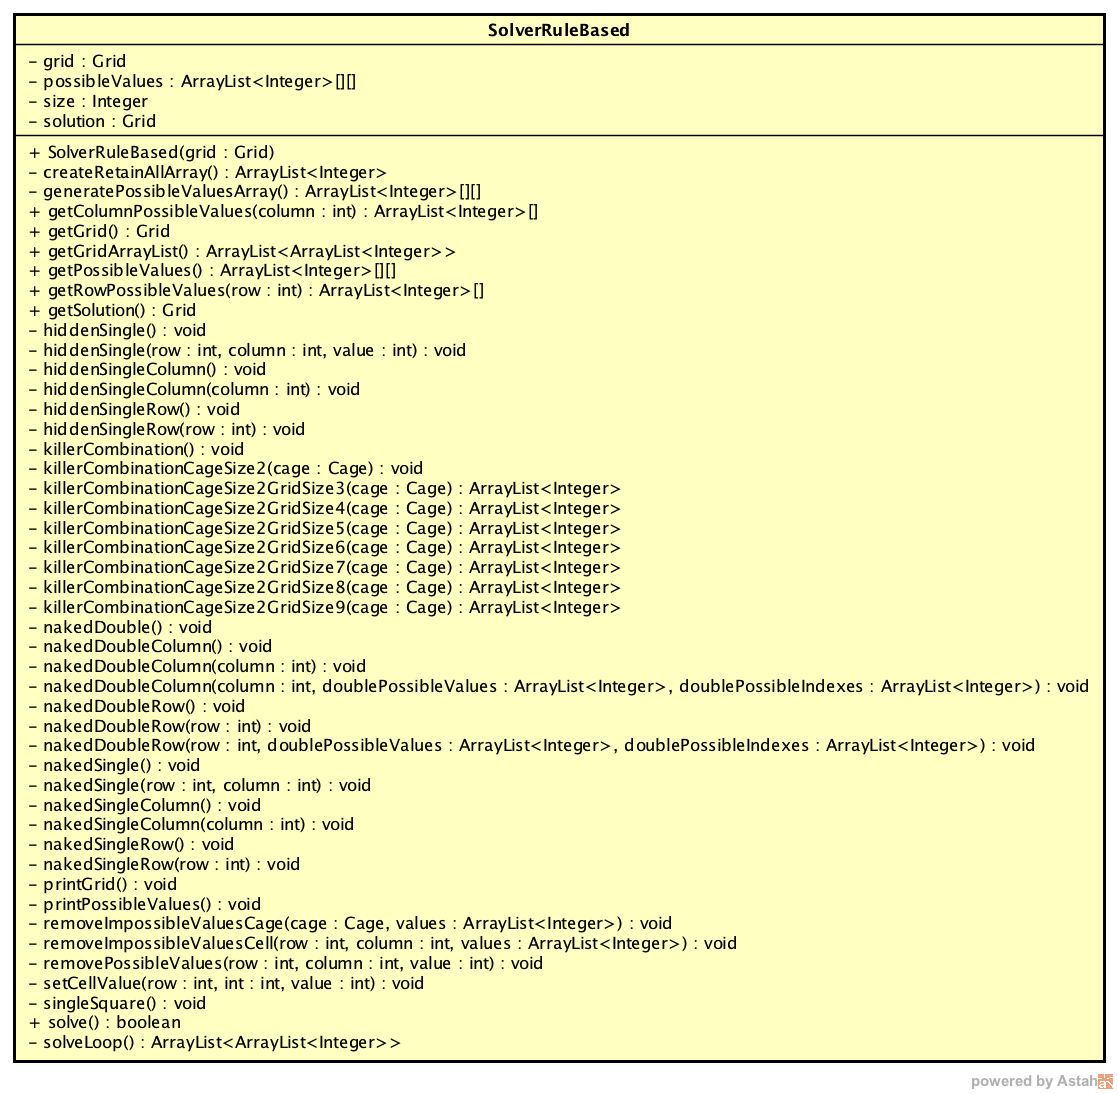
\includegraphics[scale=0.4]{Gambar/Perancangan/DiagramKelasSolverRuleBased.png}
\caption[Diagram kelas SolverRuleBased.]{Diagram kelas SolverRuleBased.}
\label{fig:diagramkelassolverrb}
\end{figure}

\subsection{Kelas SolverGenetic}
\label{sec:kelassolvergenetic}

Kelas SolverGenetic mempunyai atribut-atribut berikut, yaitu:

\begin{enumerate}
\item grid, yaitu \textit{grid} yang akan diselesaikan oleh \textit{solver} dengan algoritma genetik.
\item size, yaitu ukuran dari \textit{grid} yang akan diselesaikan oleh \textit{solver} dengan algoritma genetik.
\item isGridFixed, yaitu sebuah matriks yang berisi apakah sel tersebut sudah diisi oleh algoritma \textit{rule based} atau belum. Nilai dari sel yang sudah diisi oleh \textit{rule based} tidak boleh diganti atau dihapus.
\item randomGenerator, yaitu pembangkit angka acak.
\item generations, yaitu jumlah generasi maksimum yang akan dibangkitkan oleh algoritma genetik.
\item populationSize, yaitu jumlah kromosom yang akan dibangkitkan dalam sebuah generasi.
\item elitismRate, yaitu parameter tingkat \textit{elitism} dalam algoritma genetik.
\item crossoverRate, yaitu parameter tingkat kawin silang dalam algoritma genetik.
\item mutationRate, yaitu parameter tingkat mutasi dalam algoritma genetik.
\item solution, yaitu \textit{grid} yang sudah diselesaikan oleh \textit{solver} dengan algoritma genetik.
\item currentGeneration, yaitu generasi saat ini dalam algoritma genetik. Algoritma genetik akan membangkitkan generasi baru (nextGeneration), dan generasi baru ini akan menjadi generasi saat ini, dan algoritma akan membangkitkan generasi baru berikutnya.
\item nextGeneration, yaitu generasi berikutnya dalam algoritma genetik.
\end{enumerate}

Kelas SolverGenetic mempunyai \textit{method-method} berikut:

\begin{enumerate}
\item SolverGenetic(Grid grid, Integer generations, Integer populationSize, Double elitismRate, Double crossoverRate, Double mutationRate), yaitu konstruktor dari kelas ini. Konstruktor ini menerima masukan berupa \textit{grid} yang akan diselesaikan oleh \textit{solver} dengan algoritma genetik.
\item solve(), yaitu \textit{method} yang mencoba untuk menyelesaikan teka-teki Calcudoku menggunakan algoritma genetik. \textit{Method} ini menghasilkan keluaran apakah \textit{solver} berhasil menyelesaikan teka-teki Calcudoku atau tidak. Algoritma genetik berhasil menyelesaikan teka-teki Calcudoku jika ada kromosom yang nilai kelayakannya 1. \textit{Solver} akan membangkitkan generasi pertama, sedangkan generasi-generasi berikutnya akan dibangkitkan oleh \textit{method} solveLoop().
\item solveLoop(), yaitu \textit{method} yang membangkitkan generasi berikutnya dari generasi sebelumnya menggunakan operator algoritma genetik, yaitu \textit{elitism}, mutasi, dan kawin silang.
\item setParameters(int generations, int populationSize, double elitismRate, double crossoverRate, double mutationRate), yaitu \textit{method} untuk menentukan jumlah generasi maksimum, jumlah kromosom dalam satu generasi, tingkat \textit{elitism}, tingkat kawin silang, dan tingkat mutasi untuk algoritma genetik. Method ini menerima masukan berupa jumlah generasi maksimum, jumlah kromosom dalam satu generasi, tingkat \textit{elitism}, tingkat kawin silang, dan tingkat mutasi untuk algoritma genetik.
\item generateIsCellFixedArray(), yaitu \textit{method} yang membangkitkan matriks yang berisi apakah sel tersebut sudah diisi oleh algoritma \textit{rule based} atau tidak. \textit{Method} ini menghasilkan keluaran berupa sebuah matriks yang berisi apakah sel tersebut sudah diisi oleh algoritma \textit{rule based} atau tidak.
\item generatePopulation(), yaitu \textit{method} yang membangkitkan populasi kromosom awal.
\item generateChromosome(), yaitu \textit{method} yang membangkitkan sebuah kromosom. \textit{Method} ini menghasilkan keluaran berupa sebuah kromosom.
\item sortChromosomes(), yaitu \textit{method} yang mengurutkan kromosom-kromosom dalam generasi saat ini berdasarkan nilai kelayakannya.
\item randomSelection(ArrayList<Chromosome> chromosomes), yaitu \textit{method} untuk memilih sebuah kromosom dari sebuah populasi kromosom secara acak. \textit{Method} ini menerima masukan berupa ArrayList yang berisi sekumpulan kromosom dan menghasilkan keluaran berupa sebuah kromosom yang terpilih. Kromosom untuk proses kawin silang dan proses mutasi dipilih secara acak menggunakan \textit{method} ini.
\item cloneChromosome(Chromosome c), yaitu \textit{method} untuk mengkopi sebuah kromosom. Method ini menerima masukan berupa kromsom yang akan dikopi dan menghasilkan keluaran berupa kromosom baru hasil kopian dari kromosom yang dikopi tersebut.
\item crossover(Chromosome parent1, Chromosome parent2), yaitu \textit{method} yang mengaplikasikan operator kawin silang kepada dua kromosom. \textit{Method} ini menerima masukan berupa dua kromosom yang akan dikawinsilangkan dan menghasilkan keluaran berupa sebuah ArrayList yang berisi dua kromosom hasil kawin silang.
\item mutation(Chromosome parent), yaitu \textit{method} yang mengaplikasikan operator mutasi kepada sebuah kromosom. \textit{Method} ini menerima masukan berupa kromosom yang akan dimutasi dan menghasilkan keluaran berupa sebuah kromosom hasil mutasi.
\item getGrid, yaitu \textit{method} untuk mendapatkan \textit{grid}. Method ini menghasilkan keluaran berupa \textit{grid}.
\item getSolution, yaitu \textit{method} untuk mendapatkan \textit{grid} yang sudah diselesaikan oleh algoritma genetik. \textit{Method} ini menghasilkan keluaran berupa \textit{grid} yang sudah diselesaikan oleh algoritma genetik.
\item printGrid(), yaitu \textit{method} untuk mencetak isi \textit{grid} ke layar.
\end{enumerate}

Diagram kelas SolverGenetic dapat dilihat pada Gambar~\ref{fig:diagramkelassolvergenetic}.

\begin{figure}
\centering
\captionsetup{justification=centering}
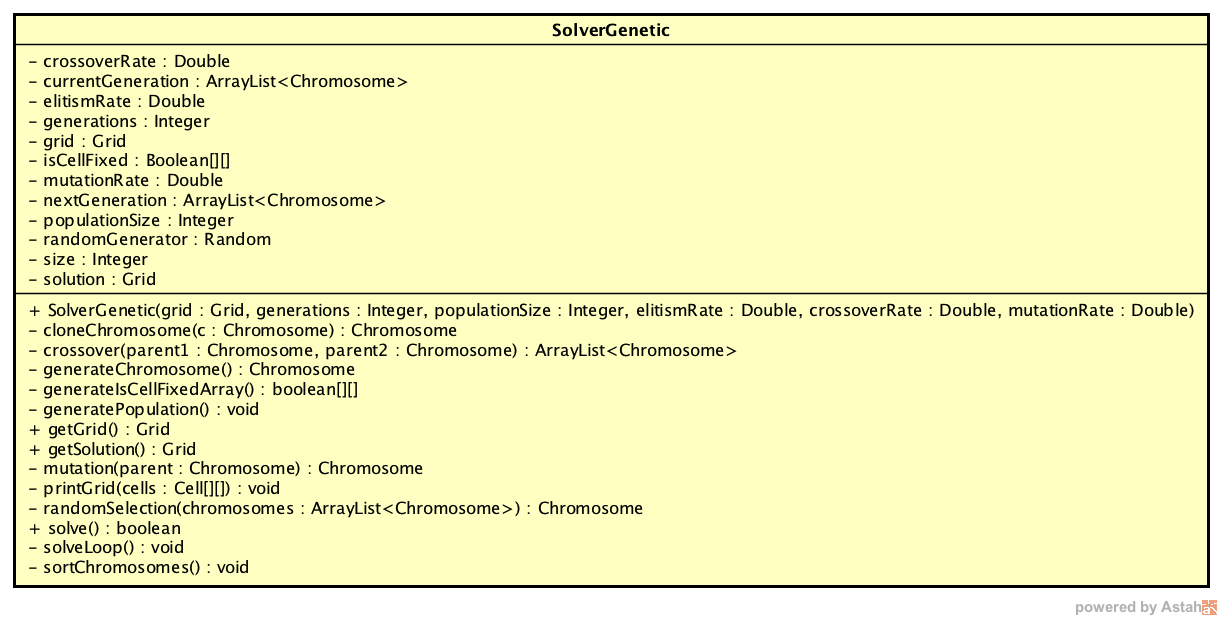
\includegraphics[scale=0.3]{Gambar/Perancangan/DiagramKelasSolverGenetic.png}
\caption[Diagram kelas SolverGenetic.]{Diagram kelas SolverGenetic.}
\label{fig:diagramkelassolvergenetic}
\end{figure}

\subsection{Kelas Chromosome}
\label{sec:kelaschromosome}

Kelas Chromosome mempunyai beberapa atribut, yaitu:

\begin{enumerate}
\item grid, yaitu sebuah \textit{grid} yang sudah diisi dengan angka-angka secara acak.
\item size, yaitu ukuran dari sebuah \textit{grid}.
\item fitness, yaitu nilai kelayakan dari sebuah \textit{grid}.
\end{enumerate}

Kelas Chromosome mempunyai beberapa \textit{method}, yaitu:

\begin{enumerate}
\item Chromosome(Grid grid), yaitu konstruktor dari kelas ini. Konstruktor ini menerima masukan berupa sebuah \textit{grid} yang sudah diisi dengan angka-angka secara acak.
\item setFitness(), yaitu \textit{method} yang menghitung nilai kelayakan untuk sebuah \textit{grid}. \textit{Method} ini menghasilkan keluaran berupa nilai kelayakan untuk \textit{grid} tersebut.
\item getFitness(), yaitu \textit{method} untuk mendapatkan nilai kelayakan untuk sebuah \textit{grid}. \textit{Method} ini menghasilkan keluaran berupa nilai kelayakan untuk \textit{grid} tersebut.
\item getGrid, yaitu \textit{method} untuk mendapatkan \textit{grid}. Method ini menghasilkan keluaran berupa \textit{grid}.
\end{enumerate}

Diagram kelas Chromosome dapat dilihat pada Gambar~\ref{fig:diagramkelaschromosome}.

\begin{figure}
\centering
\captionsetup{justification=centering}
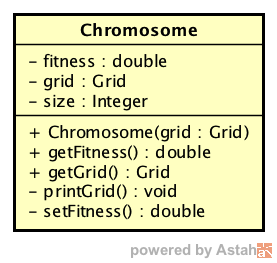
\includegraphics[scale=0.5]{Gambar/Perancangan/DiagramKelasChromosome.png}
\caption[Diagram kelas Chromosome.]{Diagram kelas Chromosome.}
\label{fig:diagramkelaschromosome}
\end{figure}

\subsection{Kelas ChromosomeComparator}
\label{sec:kelaschromosomecomparator}

Kelas ChromosomeComparator tidak mempunyai variabel, tetapi kelas ini mempunyai sebuah \textit{method}, yaitu compare(Chromosome c1, Chromosome c2). Fungsi dari \textit{method} ini adalah membandingkan dua buah kromosom berdasarkan nilai kelayakannya. \textit{Method} ini mengeluarkan hasil 1 jika c1 lebih besar daripada c2, -1 jika c1 lebih kecil daripada c2, atau 0 jika c1 sama dengan c2. Diagram kelas ChromosomeComparator dapat dilihat pada Gambar~\ref{fig:diagramkelaschromosomecomparator}.

\begin{figure}
\centering
\captionsetup{justification=centering}
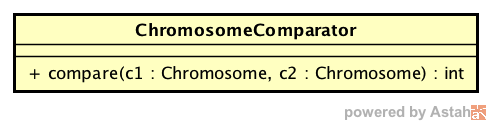
\includegraphics[scale=0.5]{Gambar/Perancangan/DiagramKelasChromosomeComparator.png}
\caption[Diagram kelas ChromosomeComparator.]{Diagram kelas ChromosomeComparator.}
\label{fig:diagramkelaschromosomecomparator}
\end{figure}

\subsection{Kelas Controller}
\label{sec:kelascontroller}

Kelas Controller mempunyai beberapa satu atribut, yaitu g. g adalah representasi dari \textit{grid} dalam teka-teki Calcudoku. grid adalah sebuah matriks yang berisi sel-sel. Matriks ini berukuran \begin{math} n \times n\end{math}.

Kelas Controller mempunyai beberapa \textit{method}, yaitu:

\begin{enumerate}
\item Controller(Integer size, Integer numberOfCages, Integer[][] cageCells, String[] cageObjectives), yaitu konstruktor dari kelas ini. Konstruktor ini menerima masukan berupa ukuran dari matriks \textit{grid}, banyaknya \textit{cage} yang terdapat dalam \textit{grid}, matriks \textit{cage assignment}, dan array \textit{cage objectives}.
\item setCellValue(int row, int column, Integer value), yaitu \textit{method} untuk mengisi sebuah sel dengan nilai yang telah ditentukan. \textit{Method} ini menerima masukan berupa nomor baris dan nomor kolom dari sel yang akan diisi dan nilai dari sel tersebut, dan menghasilkan keluaran apakah nilai dari sel tersebut \textit{valid} atau tidak. Nilai dari sebuah sel \textit{valid} jika nilai dari sel tersebut tidak berulang dalam baris dan kolom tempat sel tersebut berada, dan angka-angka dari \textit{cage} yang berisi sel tersebut mencapai angka tujuan yang telah ditentukan jika dihitung menggunakan operator yang telah ditentukan.
\item unsetCellValue(int row, int column), yaitu \textit{method} untuk menghapus isi dari sebuah sel. \textit{Method} ini menerima masukan berupa nomor baris dan nomor kolom dari sel yang akan dihapus isinya.
\item checkGrid(), yaitu \textit{method} yang memeriksa apakah ada sel yang berisi nilai yang tidak \textit{valid} atau tidak. \textit{Method} ini akan menghasilkan apakah ada sel yang berisi nilai yang tidak \textit{valid} atau tidak. \textit{Method} ini hanya bekerja jika semua sel yang berada di dalam \textit{grid} sudah diisi. Nilai dari sebuah sel \textit{valid} jika nilai dari sel tersebut tidak berulang dalam baris dan kolom tempat sel tersebut berada, dan angka-angka dari \textit{cage} yang berisi sel tersebut mencapai angka tujuan yang telah ditentukan jika dihitung menggunakan operator yang telah ditentukan.
\item getCellValue(int row, int column), yaitu \textit{method} untuk mendapatkan isi dari sebuah sel. \textit{Method} ini menerima masukan berupa nomor baris dan nomor kolom dari sel yang diminta dan menghasilkan keluaran berupa isi dari sel yang diminta tersebut.
\item getSize(), yaitu \textit{method} untuk mendapatkan ukuran dari \textit{grid}. \textit{Method} ini menghasilkan keluaran berupa ukuran dari \textit{grid}.
\item getNumberOfCages(), yaitu \textit{method} untuk mendapatkan jumlah \textit{cage} yang ada di dalam \textit{grid}. \textit{Method} ini menghasilkan keluaran berupa jumlah \textit{cage} yang ada di dalam \textit{grid}.
\item getCageCells(), yaitu \textit{method} untuk mendapatkan matriks \textit{cage assignment} dari \textit{grid}. \textit{Method} ini menghasilkan keluaran berupa matriks \textit{cage assignment} dari \textit{grid}.
\item getCageObjectives(), yaitu \textit{method} untuk mendapatkan \textit{cage objectives} dari setiap \textit{cage} dalam \textit{grid}. \textit{Method} ini menghasilkan keluaran berupa sebuah array yang berisi \textit{cage objectives} dari setiap \textit{cage} dalam \textit{grid}.
\item getGridContents(), yaitu \textit{method} untuk mendapatkan nilai dari setiap sel \textit{grid}. \textit{Method} ini menghasilkan keluaran berupa sebuah matriks yang berisi nilai dari setiap sel \textit{grid}.
\item getCages(), yaitu \textit{method} untuk mendapatkan semua \textit{cage} dalam \textit{grid}. \textit{Method} ini menghasilkan keluaran berupa array yang berisi semua \textit{cage} dalam \textit{grid}.
\item getGame(), yaitu \textit{method} untuk mendapatkan instansiasi saat ini dari kelas \textit{Grid}. \textit{Method} ini menghasilkan keluara berupa instansiasi saat ini dari kelas \textit{Grid}.
\end{enumerate}

Diagram kelas Controller dapat dilihat pada Gambar~\ref{fig:diagramkelascontroller}.

\begin{figure}
\centering
\captionsetup{justification=centering}
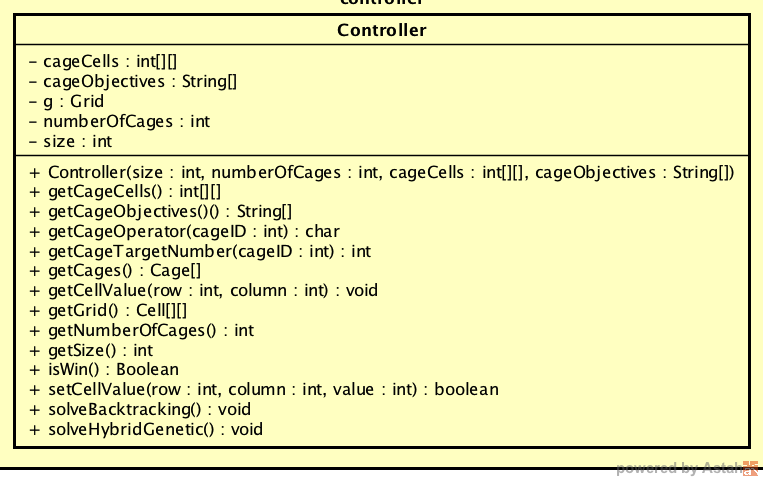
\includegraphics[scale=0.5]{Gambar/Perancangan/DiagramKelasController.png}
\caption[Diagram kelas Controller.]{Diagram kelas Controller.}
\label{fig:diagramkelascontroller}
\end{figure}

\subsection{Kelas Calcudoku}
\label{sec:kelascalcudoku}

Kelas Calcudoku mempunyai beberapa atribut, yaitu:

\begin{enumerate}
\item puzzleFile, yaitu \textit{file} permainan yang sedang dibuka oleh perangkat lunak. \textit{File} ini berbentuk \textit{file} teks.
\item size, yaitu ukuran dari matriks \textit{grid} berdasarkan \textit{file} permainan yang sedang dibuka.
\item numberOfCages, yaitu banyaknya \textit{cage} yang terdapat dalam \textit{grid} berdasarkan \textit{file} permainan yang sedang dibuka.
\item cageCells, yaitu sebuah matriks \textit{cage assignment} berdasarkan \textit{file} permainan yang sedang dibuka. Matriks ini merepresentasikan posisi dari setiap \textit{cage} dalam \textit{grid}.
\item cageObjectives, yaitu sebuah \textit{array} yang berisi \textit{cage objectives} untuk setiap \textit{cage} berdasarkan \textit{file} permainan yang sedang dibuka. \textit{Cage objectives} berisikan angka tujuan dan operasi matematika yang telah ditentukan.
\item c, yaitu sebuah instansiasi dari kelas Controller. c berfungsi untuk menghubungkan kelas-kelas yang berada di dalam \textit{package} model dengan kelas-kelas yang berada di dalam \textit{package} view.
\item menuBar, yaitu menu \textit{bar} untuk perangkat lunak ini.
\item menuFile, yaitu menu File di dalam menu \textit{bar}.
\item menuSolve, yaitu menu Solve di dalam menu \textit{bar}.
\item menuItemLoad, yaitu menu \textit{item} Load Puzzle File di dalam menu File.
\item menuItemReset, yaitu menu \textit{item} Reset Puzzle di dalam menu File.
\item menuItemClose, yaitu menu \textit{item} Close Puzzle File di dalam menu File.
\item menuItemCheck, yaitu menu \textit{item} Check Puzzle di dalam menu File.
\item menuItemExit, yaitu menu \textit{item} Exit di dalam menu File.
\item menuItemBacktracking, yaitu menu \textit{item} Backtracking di dalam menu Solve.
\item menuItemHybridGenetic, yaitu menu \textit{item} Hybrid Genetic di dalam menu File.
\item fileChooser, yaitu \textit{file chooser} untuk membuka \textit{file} permainan.
\item gui, yaitu representasi GUI dari \textit{file} permainan yang sedang dibuka.
\end{enumerate}

Kelas Calcudoku mempunyai beberapa \textit{method}, yaitu:
\begin{enumerate}
\item Calcudoku(), yaitu konstruktor dari kelas ini. Konstruktor ini berfungsi untuk menginisialisi \textit{frame} GUI.
\item main(String args[]), yaitu \textit{method main} dari perangkat lunak ini. \textit{Method} ini berfungsi untuk menjalankan perangkat lunak ini.
\item initComponents(), yaitu \textit{method} untuk menginisialisasi komponen-komponen dari \textit{frame} GUI.
\item initWindowListener(), yaitu \textit{method} untuk menginisialisasi \textit{window listener} untuk \textit{frame} GUI.
\item initActionListener(), yaitu \textit{method} untuk menginisialisasi \textit{action listener} untuk setiap menu \textit{item} yang ada di dalam \textit{frame} GUI.
\item initMenu(), yaitu \textit{method} untuk menginisialisasi menu-menu dalam menu \textit{bar} untuk \textit{frame} GUI.
\item initMenuBar(), yaitu \textit{method} untuk menginisialisasi menu \textit{bar} untuk \textit{frame} GUI.
\item menuItemLoadActionPerformed(ActionEvent evt), yaitu \textit{method} yang akan dijalankan jika menu "\textit{Load Puzzle File}" dipilih. \textit{Method} ini akan membuka \textit{file chooser} dimana pengguna memilih \textit{file} permainan untuk dibuka oleh perangkat lunak. Jika perangkat lunak sudah membuka sebuah \textit{file} permainan, maka akan keluar kotak dialog "\textit{Are you sure you want to load another puzzle file?}", jika pengguna memilih "\textit{Yes}", maka \textit{file} permainan yang baru akan dibuka oleh perangkat lunak.
\item selectPuzzleFile, yaitu \textit{method} yang memeriksa apakah \textit{file} permainan yang akan dibuka \textit{valid} atau tidak. Jika perangkat lunak gagal dalam membuka \textit{file} permainan, maka akan keluar pesan peringatan "\textit{Error in loading puzzle file}". Jika \textit{file} permainan yang dibuka bukan \textit{file} teks, maka akan keluar pesan peringatan "\textit{Invalid puzzle file}". Jika \textit{file} permainan tidak ditemukan, maka akan keluar pesan peringatan "\textit{Puzzle file not found}".
\item menuItemResetActionPerformed(ActionEvent evt), yaitu \textit{method} yang akan dijalankan jika menu "\textit{Reset Puzzle}" dipilih. \textit{Method} ini akan mengeluarkan kotak dialog "\textit{Are you sure you want to reset this puzzle?}", jika pengguna memilih "\textit{Yes}", maka perangkat lunak akan me-\textit{reset} permainan. Jika perangkat lunak tidak sedang membuka \textit{file} permainan, maka akan keluar pesan peringatan "\textit{Puzzle file not loaded}".
\item menuItemCheckActionPerformed(ActionEvent evt), yaitu \textit{method} yang akan dijalankan jika menu "\textit{Check Puzzle}" dipilih. \textit{Method} ini akan memeriksa apakah ada sel yang berisi nilai yang tidak \textit{valid} atau tidak. Nilai dari sebuah sel \textit{valid} jika nilai dari sel tersebut tidak berulang dalam baris dan kolom tempat sel tersebut berada, dan angka-angka dari \textit{cage} yang berisi sel tersebut mencapai angka tujuan yang telah ditentukan jika dihitung menggunakan operator yang telah ditentukan. \textit{Method} ini juga memeriksa apakah ada sel yang kosong atau tidak. Jika perangkat lunak tidak sedang membuka \textit{file} permainan, maka akan keluar pesan peringatan "\textit{Puzzle file not loaded}".
\item menuItemCloseActionPerformed(ActionEvent evt), yaitu \textit{method} yang akan dijalankan jika menu "\textit{Close Puzzle File}" dipilih. \textit{Method} ini akan mengeluarkan kotak dialog "\textit{Are you sure you want to close this puzzle file?}", jika pengguna memilih "\textit{Yes}", maka perangkat lunak akan menutup \textit{file} permainan dan instansiasi kelas GUI berdasarkan \textit{file} permainan yang ditutup. Jika perangkat lunak tidak sedang membuka \textit{file} permainan, maka akan keluar pesan peringatan "\textit{Puzzle file not loaded}".
\item menuItemExitActionPerformed(ActionEvent evt), yaitu \textit{method} yang akan dijalankan jika menu "\textit{Exit}" dipilih. \textit{Method} ini akan mengeluarkan kotak dialog "\textit{Are you sure you want to exit this application}", jika pengguna memilih "\textit{Yes}", maka perangkat lunak akan ditutup.
\item menuItemBacktrackingActionPerformed(ActionEvent evt), yaitu \textit{method} yang akan dijalankan jika menu "\textit{Backtracking}" dijalankan. \textit{Method} ini akan mencoba menyelesaikan permainan berdasarkan \textit{file} permainan yang dibuka dengan algoritma \textit{backtracking}. Jika perangkat lunak tidak sedang membuka \textit{file} permainan, maka akan keluar pesan peringatan "\textit{Puzzle file not loaded}".
\item menuItemHybridGeneticActionPerformed(ActionEvent evt), yaitu \textit{method} yang akan dijalankan jika menu "\textit{Hybrid Genetic}" dijalankan. \textit{Method} ini akan mencoba menyelesaikan permainan berdasarkan \textit{file} permainan yang dibuka dengan algoritma \textit{hybrid genetic}. Jika perangkat lunak tidak sedang membuka \textit{file} permainan, maka akan keluar pesan peringatan "\textit{Puzzle file not loaded}".
\item menuItemGeneticParametersActionPerformed(ActionEvent evt), yaitu \textit{method} yang akan dijalankan jika menu "\textit{Set Genetic Algorithm Parameters}" dijalankan. \textit{Method} ini akan menampilkan \textit{window} baru dimana pengguna bisa mengatur parameter-parameter untuk algoritma genetik dengan mengisi \textit{form} yang disediakan pada \textit{window} tersebut. Jika perangkat lunak tidak sedang membuka \textit{file} permainan, maka akan keluar pesan peringatan "\textit{Puzzle file not loaded}".
\item loadPuzzleFile(File puzzleFile), yaitu \textit{method} yang menginisialisasi sebuah instansiasi dari kelas GUI berdasarkan \textit{file} permainan yang dibuka. \textit{Method} ini menerima masukan berupa sebuah \textit{file} permainan. Jika perangkat lunak gagal dalam membuka \textit{file} permainan, maka akan keluar pesan peringatan "\textit{Invalid puzzle file}".
\item resetFrame(), yaitu \textit{method} untuk me-\textit{reset frame} setelah menutup \textit{file} permainan. \textit{Method} ini akan menutup instansiasi kelas GUI dan menghapus isi dari variabel c dalam \textit{frame}.
\item clearVariables(), yaitu \textit{method} untuk menghapus nilai dari variabel-variabel puzzleFile, size, cageCells, numberOfCages, dan cageObjectives dalam \textit{frame}.
\item destroyFrame(), yaitu \textit{method} untuk menutup \textit{frame} saat menutup perangkat lunak. \textit{Method} ini juga akan me-\textit{reset frame} dan menghapus nilai dari semua variabel dalam \textit{frame}.
\end{enumerate}

Diagram kelas Calcudoku dapat dilihat pada Gambar~\ref{fig:diagramkelascalcudoku}.

\begin{figure}
\centering
\captionsetup{justification=centering}
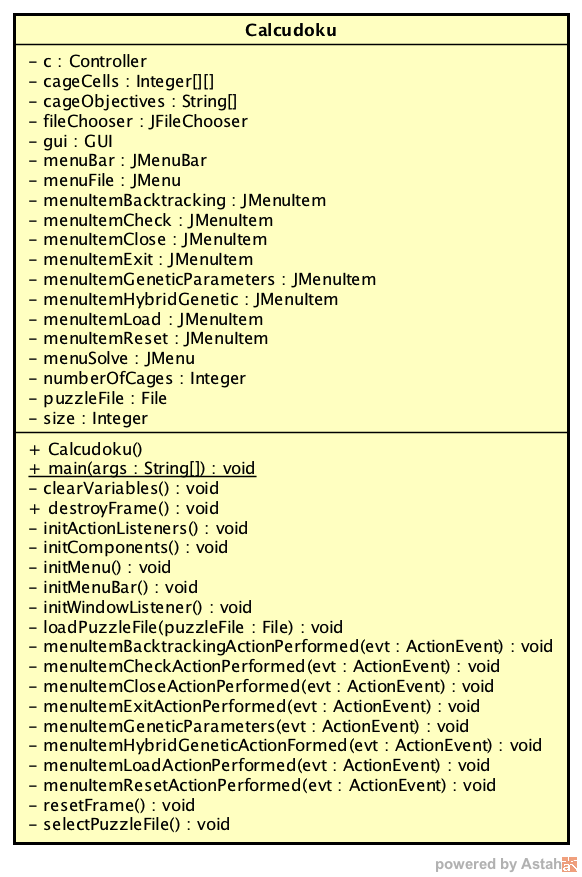
\includegraphics[scale=0.5]{Gambar/Perancangan/DiagramKelasCalcudoku.png}
\caption[Diagram kelas Calcudoku.]{Diagram kelas Calcudoku.}
\label{fig:diagramkelascalcudoku}
\end{figure}

\subsection{Kelas WindowListener}
\label{sec:kelaswindowlistener}

Kelas WindowListener hanya mempunyai satu atribut, yaitu frame. frame adalah sebuah instansiasi dari kelas Calcudoku. Kelas ini mempunya beberapa \textit{method}, yaitu:

\begin{enumerate}
\item WindowListener(Calcudoku frame), yaitu konstruktor dari kelas ini. Konstruktor ini menerima masukan berupa sebuah instansiasi dari kelas Calcudoku.
\item windowClosing(WindowEvent e), yaitu \textit{method} yang meng-\textit{override method} dari kelas WindowAdapter. \textit{Method} ini berfungsi untuk menutup semua komponen GUI saat perangkat lunak ditutup.
\item windowClosed(WindowEvent e), yaitu \textit{method} yang meng-\textit{override method} dari kelas WindowAdapter. \textit{Method} ini berfungsi untuk menutup perangkat lunak setelah semua komponen GUI ditutup.
\end{enumerate}

Diagram kelas WindowListener dapat dilihat pada Gambar~\ref{fig:diagramkelaswindowlistener}.

\begin{figure}
\centering
\captionsetup{justification=centering}
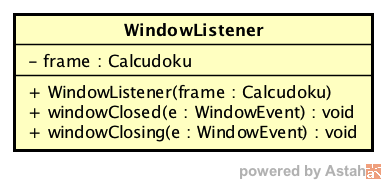
\includegraphics[scale=0.5]{Gambar/Perancangan/DiagramKelasWindowListener.png}
\caption[Diagram kelas WindowListener.]{Diagram kelas WindowListener.}
\label{fig:diagramkelaswindowlistener}
\end{figure}

\subsection{Kelas PuzzleFileFilter}
\label{sec:kelaspuzzlefilefilter}

Kelas PuzzleFileFilter tidak mempunyai atribut, tetapi memiliki beberapa \textit{method}, yaitu:

\begin{enumerate}
\item accept(File puzzleFile), yaitu \textit{method} yang meng-\textit{override method} dari kelas FileFilter. \textit{Method} ini berfungsi untuk memeriksa apakah \textit{file} yang akan dibuka memenuhi syarat atau tidak. \textit{File} yang memenuhi syarat adalah \textit{file} teks.
\item getDescription(), yaitu \textit{method} yang meng-\textit{override method} dari kelas FileFilter. \textit{Method} ini berfungsi untuk menampilkan deskripsi \textit{file} yang memenuhi syarat.
\end{enumerate}

Diagram kelas PuzzleFileFilter dapat dilihat pada Gambar~\ref{fig:diagramkelaspuzzlefilefilter}.

\begin{figure}
\centering
\captionsetup{justification=centering}
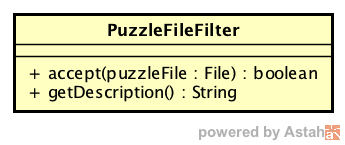
\includegraphics[scale=0.5]{Gambar/Perancangan/DiagramKelasPuzzleFileFilter.png}
\caption[Diagram kelas PuzzleFileFilter.]{Diagram kelas PuzzleFileFilter.}
\label{fig:diagramkelaspuzzlefilefilter}
\end{figure}

\subsection{Kelas GUI}
\label{sec:kelasgui}

Kelas GUI mempunyai beberapa atribut, yaitu:

\begin{enumerate}
\item c, yaitu sebuah instansiasi dari kelas Controller. c berfungsi untuk menghubungkan kelas-kelas yang berada di dalam \textit{package} model dengan kelas-kelas yang berada di dalam \textit{package} view.
\item game, yaitu sebuah instansi dari kelas Grid berdasarkan \textit{file} permainan yang sedang dibuka.
\item size, yaitu ukuran dari matriks \textit{grid} berdasarkan \textit{file} permainan yang sedang dibuka.
\item numberOfCages, yaitu banyaknya \textit{cage} yang terdapat dalam \textit{grid} berdasarkan \textit{file} permainan yang sedang dibuka.
\item cageCells, yaitu sebuah matriks \textit{cage assignment} berdasarkan \textit{file} permainan yang sedang dibuka. Matriks ini merepresentasikan posisi dari setiap \textit{cage} dalam \textit{grid}.
\item cageObjectives, yaitu sebuah \textit{array} yang berisi \textit{cage objectives} untuk setiap \textit{cage} berdasarkan \textit{file} permainan yang sedang dibuka. \textit{Cage objectives} berisikan angka tujuan dan operasi matematika yang telah ditentukan.
\item grid, yaitu sebuah \textit{array} yang berisikan semua sel yang ada di dalam \textit{grid}.
\item cages, yaitu sebuah \textit{array} yang berisikan semua \textit{cage} yang ada di dalam \textit{grid}.
\textit textFields, yaitu sebuah \textit{array} yang berisikan \textit{text field}. Setiap \textit{text field} merepresentasikan sebuah sel yang ada di dalam \textit{grid}.
\textit textFieldCoordinates, yang berfungsi untuk memetakan \textit{text field} dengan koordinat posisinya.
\textit cellTextFieldListeners, yaitu sebuah \textit{array} yang berisikan \textit{document listener} untuk semua sel yang ada di dalam \textit{grid}.
\textit font, yaitu \textit{font} yang digunakan di dalam GUI ini.
\textit cellSize, yaitu ukuran sebuah sel di dalam GUI ini.
\textit cellBorderWidth, yaitu ukuran garis pembatas antara dua sel yang berada di dalam sebuah \textit{cage} yang sama.
\textit cageBorderWidth, yaitu ukuran garis pembatas antara dua sel yang berada di dalam dua \textit{cage} yang berbeda, dan ukuran garis pembatas \textit{grid}.
\item generations, yaitu jumlah generasi maksimum yang akan dibangkitkan oleh algoritma genetik.
\item populationSize, yaitu jumlah kromosom yang akan dibangkitkan dalam sebuah generasi.
\item elitismRate, yaitu parameter tingkat \textit{elitism} dalam algoritma genetik..
\item crossoverRate, yaitu parameter tingkat kawin silang dalam algoritma genetik.
\item mutationRate, yaitu parameter tingkat mutasi dalam algoritma genetik.
\end{enumerate}

Kelas GUI mempunyai beberapa \textit{method}, yaitu:

\begin{enumerate}
\item GUI(Controller c), yaitu konstruktor dari kelas ini. Konstruktor ini berfungsi untuk menginisialisasi GUI berdasarkan \textit{file} permainan yang dibuka. \textit{Method} ini menerima masukan berupa sebuah instansiasi dari kelas Controller.
\item getController(), yaitu \textit{method} untuk mendapatkan instansiasi dari kelas Controller. \textit{Method} ini menghasilkan keluaran berupa instansiasi dari kelas Controller.
\item getGridSize(), yaitu \textit{method} untuk mendapatkan ukuran dari \textit{grid}. \textit{Method} ini menghasilkan keluaran berupa ukuran dari \textit{grid}.
\item getNumberOfCages(), yaitu \textit{method} untuk mendapatkan jumlah \textit{cage} yang ada di dalam \textit{grid}. \textit{Method} ini menghasilkan keluaran berupa jumlah \textit{cage} yang ada di dalam \textit{grid}.
\item getCageCells(), yaitu \textit{method} untuk mendapatkan matriks \textit{cage assignment} dari \textit{grid}. \textit{Method} ini menghasilkan keluaran berupa matriks \textit{cage assignment} dari \textit{grid}.
\item getCageObjectives(), yaitu \textit{method} untuk mendapatkan \textit{cage objectives} dari setiap \textit{cage} dalam \textit{grid}. \textit{Method} ini menghasilkan keluaran berupa sebuah array yang berisi \textit{cage objectives} dari setiap \textit{cage} dalam \textit{grid}.
\item getGrid(), yaitu \textit{method} untuk mendapatkan nilai dari setiap sel \textit{grid}. \textit{Method} ini menghasilkan keluaran berupa sebuah matriks yang berisi nilai dari setiap sel \textit{grid}.
\item getCages(), yaitu \textit{method} untuk mendapatkan semua \textit{cage} dalam \textit{grid}. \textit{Method} ini menghasilkan keluaran berupa array yang berisi semua \textit{cage} dalam \textit{grid}.
\item setGeneticAlgorithmParameters(Integer generations, Integer populationSize, Double elitismRate, Double crossoverRate, Double mutationRate), yaitu \textit{method} untuk mengatur parameter-parameter untuk algoritma genetik. \textit{Method} ini menerima masukan berupa jumlah generasi, jumlah populasi dalam sebuah generasi, tingkat \textit{elitism}, tingkat kawin silang, dan tingkat mutasi.
\item initTextFields, yaitu \textit{method} untuk menginisialisasi \textit{text field} yang ada di dalam \textit{grid} pada GUI.
\item solveBacktracking(), yaitu \textit{method} untuk memanggil solver untuk menyelesaikan permainan Calcudoku menggunakan algoritma \textit{backtracking}. 
\item solveHybridGenetic(), yaitu \textit{method} untuk memanggil solver untuk menyelesaikan permainan Calcudoku menggunakan algoritma \textit{hybrid genetic}.
\item printGridToScreen(), yaitu \textit{method} untuk mencetak isi \textit{grid} ke GUI.
\item clearGrid(), yaitu \textit{method} untuk menghapus isi dari semua sel yang ada di dalam \textit{grid} yang akan diselesaikan oleh \textit{solver} sebelum \textit{solver} mencoba menyelesaikan \textit{grid} tersebut.
\item addCellTextFieldListeners(), yaitu \textit{method} yang berfungsi untuk menambahkan \textit{document listener} untuk semua \textit{text field} yang ada pada GUI setelah \textit{solver} berhasil atau gagal dalam menyelesaikan permainan Calcudoku.
\item removeCellTextFieldListeners(), yaitu \textit{method} yang berfungsi untuk menghapus \textit{document listener} untuk semua \textit{text field} yang ada pada GUI sebelum \textit{solver} mencoba untuk menyelesaikan permainan Calcudoku, untuk mencegah munculnya pesan peringatan jika ada sel yang kosong atau jika ada angka yang berulang di dalam sebuah baris atau kolom.
\item moveCursor(JTextField textField), yaitu \textit{method} yang berfungsi untuk pindah dari sebuah \textit{text field} ke \textit{text field} di sebelahnya dengan menggunakan tombol-tombol panah. \textit{Method} ini menerima masukan berupa sebuah \textit{text field}.
\end{enumerate}

Diagram kelas GUI dapat dilihat pada Gambar~\ref{fig:diagramkelasgui}.

\begin{figure}
\centering
\captionsetup{justification=centering}
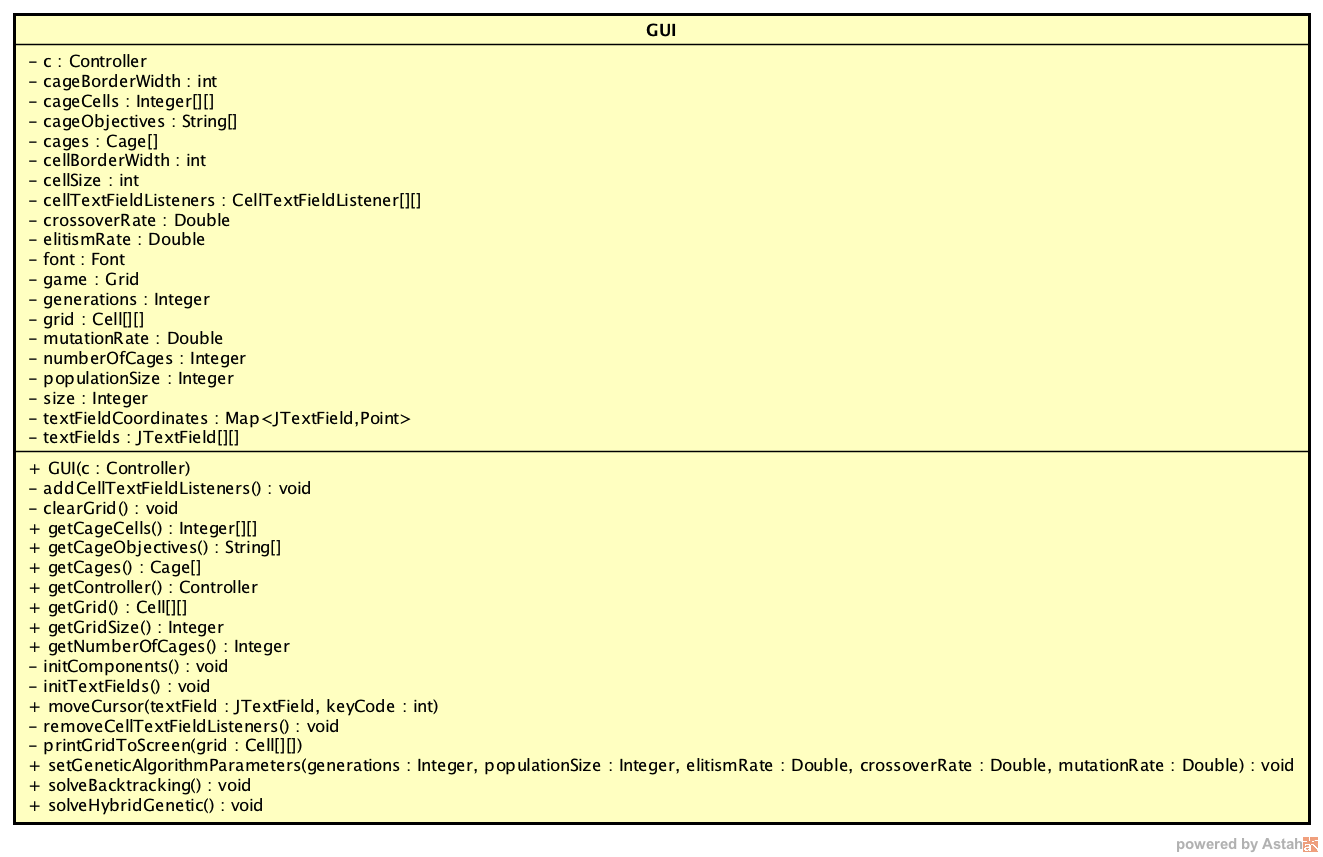
\includegraphics[scale=0.3]{Gambar/Perancangan/DiagramKelasGUI.png}
\caption[Diagram kelas GUI.]{Diagram kelas GUI.}
\label{fig:diagramkelasgui}
\end{figure}

\subsection{Kelas CellKeyListener}
\label{sec:kelascellkeylistener}

Kelas CellKeyListener hanya mempunyai satu atribut, yaitu gui. gui adalah sebuah instansiasi dari kelas GUI. Kelas ini mempunya beberapa \textit{method}, yaitu:

\begin{enumerate}
\item CellKeyLIstener(GUI gui), yaitu konstruktor dari kelas ini. Konstruktor ini menerima masukan berpua sebuah instansiasi dari kelas GUI.
\item keyPressed(KeyEvent e), yaitu \textit{method} yang meng-\textit{override method} dari kelas KeyListener. \textit{Method} ini berfungsi untuk pindah dari sebuah \textit{text field} ke \textit{text field} di sebelahnya dengan menggunakan tombol-tombol panah.
\item keyTyped(keyEvent e), yaitu \textit{method} yang meng-\textit{override method} dari kelas KeyListener. \textit{Method} ini berfungsi agar \textit{text field} hanya bisa diisi oleh sebuah angka.
\item keyReleased(keyEvent e), yaitu \textit{method} yang meng-\textit{override method} dari kelas KeyListener. \textit{Method} ini kosong.
\end{enumerate}

Diagram kelas CellKeyListener dapat dilihat pada Gambar~\ref{fig:diagramkelascellkeylistener}.

\begin{figure}
\centering
\captionsetup{justification=centering}
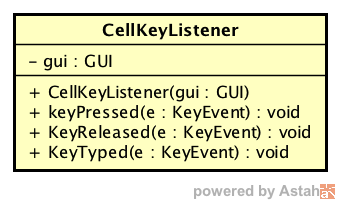
\includegraphics[scale=0.5]{Gambar/Perancangan/DiagramKelasCellKeyListener.png}
\caption[Diagram kelas CellKeyListener.]{Diagram kelas CellKeyListener.}
\label{fig:diagramkelascellkeylistener}
\end{figure}

\subsection{Kelas PopupMenuListener}
\label{sec:kelaspopupmenulistener}

Kelas PopupMenuListener mempunyai beberapa atribut, yaitu:

\begin{enumerate}
\item textField, yaitu sebuah \textit{text field} yang merepresentasikan sebuah sel yang berada di dalam \textit{grid}.
\item number, yaitu sebuah angka.
\end{enumerate}

\clearpage

Kelas PopupMenuListener mempunyai beberapa \textit{method}, yaitu:

\begin{enumerate}
\item PopupMenuListener(JTextField textField, int number), yaitu konstruktor dari kelas ini. Konstruktor ini menerima masukan berupa sebuah \textit{text field} dan sebuah angka.
\item actionPerformed(ActionEvent e), yaitu \textit{method} yang meng-\textit{override method} dari kelas ActionListener. \textit{Method} ini berfungsi untuk mengisi sebuah \textit{text field} dengan angka yang dipilih.
\end{enumerate}

Diagram kelas PopupMenuListener dapat dilihat pada Gambar~\ref{fig:diagramkelaspopupmenulistener}.

\begin{figure}
\centering
\captionsetup{justification=centering}
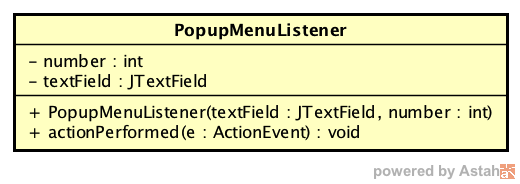
\includegraphics[scale=0.5]{Gambar/Perancangan/DiagramKelasPopupMenuListener.png}
\caption[Diagram kelas PopupMenuListener.]{Diagram kelas PopupMenuListener.}
\label{fig:diagramkelaspopupmenulistener}
\end{figure}

\subsection{Kelas CellTextFieldListener}
\label{sec:kelascelltextfieldlistener}

Kelas CellTextFieldListener mempunyai beberapa atribut, yaitu:

\begin{enumerate}
\item c, yaitu sebuah instansiasi dari kelas Controller. c berfungsi untuk menghubungkan kelas-kelas yang berada di dalam \textit{package} model dengan kelas-kelas yang berada di dalam \textit{package} view.
\item textField, yaitu sebuah \textit{text field} yang merepresentasikan sebuah sel yang berada di dalam \textit{grid}.
\item x, yaitu koordinat x dari \textit{text field}.
\item y, yaitu koordinat y dari \textit{text field}.
\end{enumerate}

Kelas CellTextFieldListener mempunyai beberapa \textit{method}, yaitu:

\begin{enumerate}
\item CellTextFieldListener(Controller c, JTextField textField, int x, int y), yaitu konstruktor dari kelas ini. Konstruktor ini menerima masukan berupa sebuah instansiasi dari kelas Controller, sebuah \textit{text field}, dan koordinat dari \textit{text field} tersebut.
\item insertUpdate(DocumentEvent e), yaitu \textit{method} yang meng-\textit{override method} dari kelas DocumentEvent. \textit{Method} ini berfungsi untuk mengisi sebuah sel pada kelas Grid dengan angka yang diisikan ke dalam sel pada GUI.
\item removeUpdate(DocumentEvent e), yaitu \textit{method} yang meng-\textit{override method} dari kelas DocumentEvent. \textit{Method} ini berfungsi untuk menghapus isi sebuah sel pada kelas Grid jika angka dalam sel pada GUI dihapus.
\item changeUpdate(DocumentEvent e), yaitu \textit{method} yang meng-\textit{override method} dari kelas DocumentEvent. \textit{Method} ini berfungsi untuk menghapus isi sebuah sel pada kelas Grid dan mengisi sebuah sel pada kelas Grid dengan angka yang baru yang diisikan ke dalam sel pada GUI jika terjadi perubahan angka yang diisikan ke dalam sel pada GUI.
\end{enumerate}

Diagram kelas CellTextFieldListener dapat dilihat pada Gambar~\ref{fig:diagramkelascelltextfieldlistener}.

\begin{figure}
\centering
\captionsetup{justification=centering}
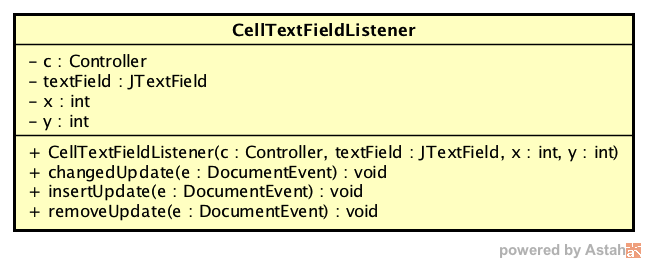
\includegraphics[scale=0.5]{Gambar/Perancangan/DiagramKelasCellTextFieldListener.png}
\caption[Diagram kelas CellTextFieldListener.]{Diagram kelas CellTextFieldListner.}
\label{fig:diagramkelascelltextfieldlistener}
\end{figure}

\subsection{Kelas GeneticParameters}
\label{sec:kelasgeneticparamater}

Kelas GeneticParameters mempunyai beberapa atribut, yaitu:

\begin{enumerate}
\item gui, yaitu representasi GUI dari \textit{file} permainan yang sedang dibuka.
\item labelGenerations, yaitu label yang bertuliskan "\textit{Generations}".
\item labelPopulation, yaitu label yang bertuliskan "\textit{Population Size}".
\item labelElitism, yaitu label yang bertuliskan "\textit{Elitism Rate}".
\item labelCrossover, yaitu label yang bertuliskan "\textit{Crossover Rate}".
\item labelMutation, yaitu label yang bertuliskan "\textit{Mutation Rate}".
\item textFieldGenerations, yaitu \textit{text field} untuk mengisi nilai jumlah generasi.
\item textFieldPopulation, yaitu \textit{text field} untuk mengisi nilai jumlah populasi dalam sebuah generasi.
\item textFieldElitism, yaitu \textit{text field} untuk mengisi nilai tingkat \textit{elitism}.
\item textFieldCrossover, yaitu \textit{text field} untuk mengisi nilai tingkat kawin silang.
\item textFieldMutation, yaitu \textit{text field} untuk mengisi nilai tingkat mutasi.
\item buttonOK, yaitu tombol untuk mengganti nilai-nilai parameter untuk algoritma genetik dengan nilai-nilai yang dimasukkan ke dalam \textit{form} yang disediakan.
\item buttonCancel, yaitu tombol untuk membatalkan perubahan nilai-nilai parameter untuk algoritma genetik.
\end{enumerate}

Kelas GeneticParameters mempunyai beberapa \textit{method}, yaitu:

\begin{enumerate}
\item GeneticParameterss(GUI gui), yaitu konstruktor dari kelas ini. Konstruktor ini menerima masukan berpua sebuah instansiasi dari kelas GUI.
\item initComponents(), yaitu \textit{method} untuk menginisialisasi komponen-komponen dari \textit{form}.
\item initActionListener(), yaitu \textit{method} untuk menginisialisasi \textit{action listener} untuk setiap tombol yang ada di dalam \textit{form}.
\item initGUI(), yaitu \textit{method} untuk menginisialisasi GUI dari \textit{form}.
\item initMenuBar(), yaitu \textit{method} untuk menginisialisasi menu \textit{bar} untuk \textit{frame} GUI.
\item buttonOKActionPerformed(ActionEvent evt), yaitu \textit{method} yang akan dijalankan jika tombol "\textit{OK}" ditekan. \textit{Method} ini akan mengganti nilai-nilai parameter untuk algoritma genetik dengan nilai-nilai yang telah dimasukkan ke dalam \textit{form} yang disediakan.
\item buttonCancelActionPerformed(ActionEvent evt), yaitu \textit{method} yang akan dijalankan jika tombol "\textit{Cancel}" ditekan. \textit{Method} ini akan membatalkan perubahan nilai-nilai parameter untuk algoritma genetik.
\item destroyFrame(), yaitu \textit{method} untuk menutup \textit{form}.
\end{enumerate}

Diagram kelas GeneticParameters dapat dilihat pada Gambar~\ref{fig:diagramkelasgeneticparameters}.

\begin{figure}
\centering
\captionsetup{justification=centering}
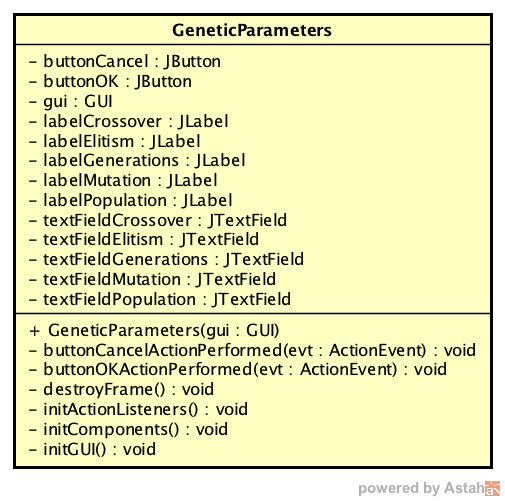
\includegraphics[scale=0.5]{Gambar/Perancangan/DiagramKelasGeneticParameters.png}
\caption[Diagram kelas GeneticParameters.]{Diagram kelas GeneticParameters.}
\label{fig:diagramkelasgeneticparameters}
\end{figure}